%%%%%%%%%%%%%%%%%%%%%%% file template.tex %%%%%%%%%%%%%%%%%%%%%%%%%
%
% This is a general template file for the LaTeX package SVJour3
% for Springer journals.          Springer Heidelberg 2010/09/16
%
% Copy it to a new file with a new name and use it as the basis
% for your article. Delete % signs as needed.
%
% This template includes a few options for different layouts and
% content for various journals. Please consult a previous issue of
% your journal as needed.
%
%%%%%%%%%%%%%%%%%%%%%%%%%%%%%%%%%%%%%%%%%%%%%%%%%%%%%%%%%%%%%%%%%%%
%
% First comes an example EPS file -- just ignore it and
% proceed on the \documentclass line
% your LaTeX will extract the file if required
\begin{filecontents*}{example.eps}
%!PS-Adobe-3.0 EPSF-3.0
%%BoundingBox: 19 19 221 221
%%CreationDate: Mon Sep 29 1997
%%Creator: programmed by hand (JK)
%%EndComments
gsave
newpath
  20 20 moveto
  20 220 lineto
  220 220 lineto
  220 20 lineto
closepath
2 setlinewidth
gsave
  .4 setgray fill
grestore
stroke
grestore
\end{filecontents*}
%
%\RequirePackage{fix-cm}
%
% \documentclass{svjour3}                     % onecolumn (standard format)
%\documentclass[smallcondensed]{svjour3}     % onecolumn (ditto)
% \documentclass[smallextended]{svjour3}       % onecolumn (second format)
\documentclass[twocolumn]{svjour3}          % twocolumn
%
\smartqed  % flush right qed marks, e.g. at end of proof
%
\usepackage{graphicx}
%
\usepackage{mathptmx}      % use Times fonts if available on your TeX system
%
% insert here the call for the packages your document requires
\usepackage{amssymb,amsmath,amsfonts,mathtools}
\usepackage{hyperref} 
\usepackage{algorithm}
\usepackage{algpseudocode}
\usepackage{color}
\alglanguage{pseudocode}
\usepackage{tikz}
\usetikzlibrary{arrows}
%\usepackage[british]{babel}
% \usepackage{draftwatermark}
% \SetWatermarkText{DRAFT}
% \SetWatermarkScale{1}

\definecolor{darkgray}{rgb}{0.66, 0.66, 0.66}
\definecolor{arsenic}{rgb}{0.23, 0.27, 0.29}
\definecolor{dimgray}{rgb}{0.41, 0.41, 0.41}
% \definecolor{lightgray}{\colorlet{shadecolor}{gray!40}}

\usepackage{epstopdf}
\epstopdfsetup{update}

\usepackage{caption}
\usepackage{subcaption}
\usepackage{ragged2e} 

% \usepackage{etoolbox}
% \newrobustcmd*{\mytriangle}[1]{\tikz{\filldraw[draw=#1,fill=#1] (0,0.2cm) -- (0.2cm,0.2cm) -- (0.1cm,0);}}

%Laplace symbol
\newcommand*\Laplace{\mathop{}\!\mathbin\bigtriangleup}

\newcommand{\vv}[1]{\mathbf{#1}}
\newcommand{\trp}{\mathsf{H}}
\newcommand{\overbar}[1]{\mkern 1.5mu\overline{\mkern-1.5mu#1\mkern-1.5mu}\mkern 1.5mu}

%right hand size vector
\newcommand{\rhs}{\mathbf{b}}
\newcommand{\source}{\mathbf{s}}
%right hand size block vector
\newcommand{\blkrhs}{B}

%main operator A
\newcommand{\op}{{\mathcal{A}}}
%Preconditioning operator P
\newcommand{\precon}{{\mathcal{P}}}

% scalar shift
\newcommand{\shift}{{\omega}}
%G_j parameter in IDR
\newcommand{\idrpar}{{\xi}}
%leading dimension of A
\newcommand{\n}{N}
%Number of shift
\newcommand{\Nom}{{N_\shift}}
% Spatial dimensions
\newcommand{\nx}{{n_x}}
\newcommand{\ny}{{n_y}}
\newcommand{\nz}{{n_z}}
% Number of blocks D_i
\newcommand{\nblks}{{n}}
\newcommand{\ssorfac}{{\eta}}

%R set
\newcommand{\R}{{\mathbb{R}}}
%C set
\newcommand{\C}{{\mathbb{C}}}
%shadow space for IDR
\newcommand{\shadow}{{\mathcal{S}}}

%Unknow 
\newcommand{\x}{{\mathbf{x}}}
\newcommand{\X}{{\mathbf{X}}}

% mathcal soooo ugly
\newcommand{\sss}{SSS }
\newcommand{\msss}{MSSS }
\newcommand{\rank}{{r}}

\newcommand{\marmousi}{\texttt{Marmousi-II} }

\makeatletter
\providecommand*{\cupdot}{%
  \mathbin{%
    \mathpalette\@cupdot{}%
  }%
}
\newcommand*{\@cupdot}[2]{%
  \ooalign{%
    $\m@th#1\cup$\cr
    \hidewidth$\m@th#1\cdot$\hidewidth
  }%
}
\makeatother

\def\ds{\displaystyle} 

\newtheorem{exper}{Experiment}


\begin{document}


\title{An MSSS-Preconditioned Matrix Equation Approach for the Time-Harmonic Elastic Wave Equation at Multiple Frequencies}
% \subtitle{Do you have a subtitle?\\ If so, write it here}
% \titlerunning{An MSSS preconditioner for the time-harmonic elastic wave equation at multiple frequencies}        % if too long for running head

\author{M. Baumann \and R. Astudillo \and Y. Qiu \and E. Ang \and M.B. van Gijzen \and R.-\'E. Plessix}

%\authorrunning{Short form of author list} % if too long for running head
% Commented for the Technical Report
\institute{Manuel Baumann (corresponding)\at
           Delft University of Technology\\
           Delft Institute of Applied Mathematics\\
           \email{\href{m.m.baumann@tudelft.nl}{\texttt{m.m.baumann@tudelft.nl}}}
           \and
           Reinaldo Astudillo \at
           Delft University of Technology
	   \and
           Yue Qiu \at
           Max Planck Institute for Dynamics \\of Complex Technical Systems
           \and
           Elisa Ang \at
           Nanyang Technological University
           \and
           Martin B. van Gijzen\at
           Delft University of Technology
           \and
           Ren\'e-\'Edouard Plessix \at
           Shell Global Solutions International B.V.
}

\date{\today}
% The correct dates will be entered by the editor

\maketitle

\begin{abstract}
In this work we present a new numerical framework for the efficient solution of the time-harmonic elastic wave equation at multiple frequencies. We show that multiple frequencies (and multiple right-hand sides) can be incorporated when the discretized problem is written as a matrix equation. This matrix equation can be solved efficiently using the preconditioned IDR($s$) method. We present an efficient and robust way to apply a single preconditioner using MSSS matrix computations. For 3D problems, we present a memory-efficient implementation that exploits the solution of a sequence of 2D problems. Realistic examples in two and three spatial dimensions demonstrate the performance of the new algorithm.

\keywords{time-harmonic elastic wave equation \and multiple frequencies \and Induced Dimension Reduction (IDR) method \and preconditioned matrix equations \and multilevel sequentially semiseparable matrices (MSSS)}
% \PACS{PACS code1 \and PACS code2 \and more}
% \subclass{MSC code1 \and MSC code2 \and more}
\end{abstract}

% \tableofcontents

\section{Introduction}
\label{intro}
% The understanding of the earth subsurface is a key task in geophysics, and seismic exploration is an approach that match\-es the intensity of reflected shock waves with simulation results in a least squares sense; cf. \cite{VO09} and the references therein for an overview of state-of-the-art Full-Waveform Inversion (FWI) algorithms. 
The understanding of the earth subsurface is a key task in geophysics, and Full-Waveform Inversion (FWI) is a computational approach that match\-es the intensity of reflected shock waves (measurements) with simulation results in a least squares sense; cf. \cite{VO09} and the references therein for an overview of state-of-the-art FWI algorithms. From a mathematical point of view, the problem of matching measurements with simulation results leads to a PDE-constrained optimization problem where the objective function is defined by the respective FWI approach, and the constraining partial differential equation (PDE) is the wave equation. Since the earth is an elastic medium, the elastic wave equation needs to be considered. In order to design an efficient optimization algorithm, a fast numerical solution of the elastic wave equation is required at every iteration of the optimization loop. This so-called \textit{forward problem} is the focus of this work.

More recently, FWI has been considered for an equivalent problem formulated in the frequency-domain \cite{MPl04,P99}. The frequency-domain formulation of wave propagation has shown specific modeling advantages for both acoustic and elastic media. For the efficient FWI, notably the waveform tomography \cite{PPS15,VO09}, a fast numerical solution of the respective time-harmonic forward problem is required. More precisely, the forward problem requires the fast numerical solution of the discretized time-harmonic elastic wave equation at multiple wave frequencies and for multiple source terms. In this context, many efficient numerical solution methods have been proposed mostly for the (acoustic) Helmholtz e\-qua\-tion \cite{PN14,P09,PM04,REPMVO06}. In this work, we present an efficient solver of the time-harmonic \textit{elastic} wave equation that results from a finite element discretization, cf. \cite{DBD09,ECVG10}. 

Especially for large 3D problems, the efficient numerical solution with respect to computation time and memory requirements is subject to current research. When an iterative Krylov method is considered, the design of efficient preconditioners for the elastic wave equation is required. In \cite{apt09} a damped preconditioner for the elastic wave equation is presented. The authors of \cite{Rizzuti2016} analyze a multi-grid approach for the damped problem. Both works are extensions of the work of Erlangga et al. \cite{REPMVO06} for the acoustic case. The recent low-rank approach of the MUMPS solver \cite{Amestoy2015} makes use of the hierarchical structure of the discrete problem and can be used as a preconditioner, cf. \cite{ABBEMMMO16,WHXL12}. When domain decomposition is considered, the sweeping preconditioner \cite{Tsuji2014} is an attractive alternative.

In this work we propose a \textit{hybrid} method that combines the iterative Induced Dimension Reduction (IDR) method with an efficient preconditioner that exploits the multilevel sequentially semiseparable (MSSS) matrix structure of the discretized elastic wave equation on a Cartesian grid. Moreover, we derive a matrix equation formulation that includes multiple frequencies and multiple right-hand sides, and pres\-ent a version of IDR that solves linear matrix equations at a low memory requirement. The paper is structured as follows: In Section \ref{sec:EWE}, we derive a finite element discretization for the time-har\-mon\-ic elastic wave equation with a special emphasis on the case when multiple frequencies are present. Section \ref{ch:idr} pres\-ents the IDR($s$) method for the iterative solution of the resulting matrix equation. We discuss an efficient preconditioner in Section \ref{ch:msss} based on the MSSS structure of the discrete problem. We present different versions of the MSSS preconditioner for 2D and 3D problems in Section \ref{ch:msss_lu} and \ref{ch_msss3d}, respectively. The paper concludes with extensive numerical tests in Section \ref{ch:num}.

\section{The time-harmonic elastic wave equation at multiple frequencies}
\label{sec:EWE}
In this section we present a finite element discretization of the time-harmonic elastic wave equation with a special emphasis on the mathematical and numerical treatment when multiple frequencies (and possibly multiple right-hand sides) are present.

\subsection{Problem description}
 The time-harmonic elastic wave equation describes the displacement vector $\mathbf{u}:\Omega \rightarrow \mathbb{C}^d$ in a computational domain $\Omega \subset \mathbb{R}^{d}, d \in \{2,3\},$ governed by the following partial differential equation (PDE),
 \begin{align}
 \label{LEWE}
 -\shift_k^2 \rho(\mathbf{x}) \mathbf{u}_k - \nabla \! \cdot \! \sigma(\mathbf{u}_k) = \source , \ \mathbf{x} \in \Omega \subset \mathbb{R}^{d}, \ k=1,...,\Nom.
\end{align}

Here, $\rho(\mathbf{x})$ is the density of an elastic material in the considered domain $\Omega$ that can differ with $\mathbf{x} \in \Omega$ (inhomogeneity), $\source$ is a source term, and $\{\shift_1,...,\shift_\Nom\}$ are multiple angular frequencies that define $\Nom$ problems in \eqref{LEWE}. The stress and strain tensor follow from Hooke's law for isotropic elastic media,
\begin{align}
\label{eq:Hook}
 \sigma(\mathbf{u}_k) &:= \lambda(\mathbf{x}) \left( \nabla \! \cdot \! \mathbf{u}_k \ I_d \right) + 2 \mu(\mathbf{x}) \epsilon(\mathbf{u}_k), \\
 \epsilon(\mathbf{u}_k) &:= \frac{1}{2} \left( \nabla \mathbf{u}_k + \left( \nabla \mathbf{u}_k\right)^\mathsf{T} \right),
\end{align}
  with $\lambda, \mu$ being the Lam\'e parameters \eqref{eq:lame}. On the boundary $\partial \! \Omega$ of the domain $\Omega$, we consider the following boundary conditions,
\begin{align}
i \shift_k \rho(\mathbf{x}) B \mathbf{u}_k + \sigma(\mathbf{u}_k)\mathbf{\hat n} = \mathbf{0}, \quad \mathbf{x} \in \partial \! \Omega_a, \label{bc1}\\
\sigma(\mathbf{u}_k)\mathbf{\hat n} = \mathbf{0}, \quad \mathbf{x} \in \partial \! \Omega_r, \label{bc2}
\end{align}
where Sommerfeld radiation boundary conditions at $\partial \! \Omega_a$ model absorption, and we typically prescribe a free-surface bound\-a\-ry condition in the north of the computational domain $\partial \! \Omega_r$, with $\partial \! \Omega_a \cupdot \partial \! \Omega_r = \partial \! \Omega$. In \eqref{bc1}, $B$ is a $d \times d$ matrix that depends on $c_p$ and $c_s$, $\quad B \equiv B(\mathbf{x}) := c_p(\mathbf{x}) \mathbf{\hat n} \mathbf{\hat n}^\mathsf{T} + c_s(\mathbf{x}) \mathbf{\hat t} \mathbf{\hat t}^\mathsf{T} + c_s(\mathbf{x}) \mathbf{\hat s} \mathbf{\hat s}^\mathsf{T}$, with vectors $\{\mathbf{\hat n},\mathbf{\hat t},\mathbf{\hat s}\}$ being normal or tangential to the bound\-a\-ry, respectively; cf. \cite{apt09} for more details. Note that the boundary conditions \eqref{bc1}-\eqref{bc2} can naturally be included in a finite element approach as explained in Section \ref{ch:discretization}.
\begin{figure}[ht]
\centering
\vspace{-0.3cm}
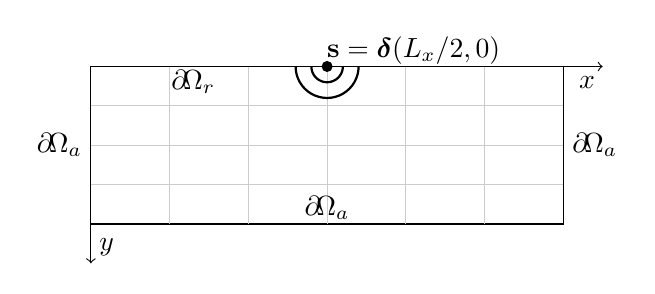
\begin{tikzpicture}
 \draw (0,0) -- (6,0) -- (6,2) -- (0,2) -- (0,0);
%  \draw (0,1) -- (4,1);
%  \draw (0,2) -- (4,2);
%  \draw (1,0) -- (1,3);
%  \draw (2,0) -- (2,3);
%  \draw (3,0) -- (3,3);

  \draw[gray!40] (0,0.5) -- (6,0.5);
  \draw[gray!40] (0,1) -- (6,1);
  \draw[gray!40] (0,1.5) -- (6,1.5);
  
  \draw[gray!40] (1,0) -- (1,2);
  \draw[gray!40] (2,0) -- (2,2);
  \draw[gray!40] (3,0) -- (3,2);
  \draw[gray!40] (4,0) -- (4,2);
  \draw[gray!40] (5,0) -- (5,2);
 
 \draw[->] (0,2) -- (6.5,2);
 \node at (6.3,1.8) {$x$};
 \draw[->] (0,2) -- (0,-0.5);
 \node at (0.2,-0.3) {$y$};
 
 \draw [thick,domain=180:360] plot ({3+0.2*cos(\x)}, {2+0.2*sin(\x)});
 \draw [thick,domain=180:360] plot ({3+0.4*cos(\x)}, {2+0.4*sin(\x)});
 \fill (3,2) circle[radius=2pt];
 
%  \fill (0,0) circle[radius=2pt];
%  \fill (1,0) circle[radius=2pt];
%  \fill (2,0) circle[radius=2pt];
%  \fill (3,0) circle[radius=2pt];
%  \fill (4,0) circle[radius=2pt];
%  \fill (0,1) circle[radius=2pt];
%  \fill (1,1) circle[radius=2pt];
%  \fill (2,1) circle[radius=2pt];
%  \fill (3,1) circle[radius=2pt];
%  \fill (4,1) circle[radius=2pt];
%  \fill (0,2) circle[radius=2pt];
%  \fill (1,2) circle[radius=2pt];
%  \fill (2,2) circle[radius=2pt];
%  \fill (3,2) circle[radius=2pt];
%  \fill (4,2) circle[radius=2pt];
%  \fill (0,3) circle[radius=2pt];
%  \fill (1,3) circle[radius=2pt];
%  \fill (3,3) circle[radius=2pt];
%  \fill (4,3) circle[radius=2pt];

 \node at (-0.4,1) {$\partial \! \Omega_a$};
 \node at (6.4,1) {$\partial \! \Omega_a$};
 \node at (3,0.2) {$\partial \! \Omega_a$};
 \node at (1.3,1.8) {$\partial \! \Omega_r$};
 
 \node at (4.1,2.2) {$\source = \boldsymbol{\delta}(L_x/2,0)$}; 
\end{tikzpicture}
\caption{Boundary conditions and source term for $d=2$. For $d=3$, the source is for instance located at $(L_x/2,L_y/2,0)^\mathsf{T}$.} \label{mesh}
\end{figure}

We assume the set of five parameters $\{\rho, c_p, c_s, \lambda, \mu\}$ in \eqref{LEWE}-\eqref{bc2} to be space-dependent. The Lam\'e parameters $\lambda$ and $\mu$ are directly related to the material density $\rho$ and the speed of P-waves $c_p$ and speed of S-waves $c_s$ via,
\begin{align}
\label{eq:lame}
%   \mu = c_s^2  \rho, \quad \lambda = c_p^2 \rho - 2 \mu.% \quad \text{ in } \Omega.
  \mu = c_s^2  \rho, \quad \lambda = \rho(c_p^2 - 2 c_s^2).% \quad \text{ in } \Omega.
\end{align}
All parameter functions are assumed in $L^1(\Omega)$. More specifically, we interpolate data points using $Q_1$ basis functions. 
\subsection{Finite element (FEM) discretization}
\label{ch:discretization}
For the discretization of \eqref{LEWE}-\eqref{bc2} we follow a classical finite element approach using the following ansatz,
\begin{align}
\label{eq:ansatz}
\mathbf{u}_k(\mathbf{x}) \approx \sum_{i=1}^\n u_k^i\boldsymbol\varphi_i(\mathbf{x}), \quad \mathbf{x} \in \Omega \subset \mathbb{R}^{d}, \quad u_k^i \in \C.
\end{align}
In the numerical examples presented in Section \ref{ch:num} we restrict ourselves to Cartesian grids and basis functions $\boldsymbol\varphi_i$ that are B-splines of degree $p$ as described for instance in \cite[Chapter 2]{isoa09}. The number of degrees of freedom is, hence, given by 
\begin{align}
\label{eq:unknows}
\n = d \prod_{i \in \{x,y,z\}} (n_i-1+p), \quad d \in \{2,3\}, p \in \mathbb{N}^{+},
\end{align}
with $n_i$ grid points in the respective spatial direction (in Figure \ref{mesh} we illustrate the case where $d=2$ and $n_x=7, n_y=5$).

\begin{definition}[Tensor notation, \cite{elman2014finite}]
\label{def:inner}
 The \textit{dot product} between two vector-valued quantities $\mathbf{u} = (u_x,u_y), \mathbf{v} = (v_x,v_y)$ is denoted as,
  $\mathbf{u} \cdot \mathbf{v} := u_x v_x + u_y v_y$. Similarly, we define the \textit{componentwise multiplication} of two matrices $U = [u_{ij}], V = [v_{ij}]$ as,
  $U : V := \sum_{i,j} u_{ij}v_{ij}$.
 \end{definition}

A Galerkin finite element approach applied to \eqref{LEWE} yields the following weak form: Find $\boldsymbol \varphi_i \in [H^1(\Omega)]^d$  such that,
\begin{align*}
% -\shift_k^2 \int_\Omega \rho(\mathbf{x}) \left(\sum_i u_k^i\boldsymbol\varphi_i\right) \boldsymbol\varphi_j \ d \! \Omega  - \int_\Omega \nabla \cdot \sigma(\sum_i u_k^i\boldsymbol\varphi_i) \boldsymbol\varphi_j \ d \! \Omega \\ = \int_\Omega \mathbf{s}  \boldsymbol\varphi_j \ d \! \Omega, \quad j=1,...,N, \\
-\shift_k^2 \sum_{i=1}^N u_k^i \int_{\Omega} \rho(\mathbf{x}) \boldsymbol\varphi_i \cdot \boldsymbol\varphi_j \ d \!\Omega - \sum_{i=1}^N u_k^i \int_\Omega \nabla \! \cdot \! \sigma(\boldsymbol\varphi_i) \cdot \boldsymbol{\varphi_j} \ d \! \Omega  \\ = \int_\Omega \source \cdot \boldsymbol\varphi_j \ d \! \Omega, \quad \text{for all }  \boldsymbol \varphi_j \in [H^1(\Omega)]^d,
\end{align*}
$j=1,...,N$, and for all source functions $\mathbf{s} \in [L^1(\Omega)]^d$. We exploit the boundary conditions \eqref{bc1}-\eqref{bc2} in the following way,
\begin{align*}
 \int_\Omega \nabla \! \cdot \! \sigma(\boldsymbol\varphi_i) \cdot \boldsymbol{\varphi_j} \ d \! \Omega \\ =  \int_{\partial \! \Omega} \sigma(\boldsymbol\varphi_i) \boldsymbol\varphi_j \cdot \mathbf{\hat n} \ d \! \Gamma - \int_\Omega \sigma(\boldsymbol\varphi_i) : \nabla \boldsymbol\varphi_j \ d \! \Omega \\
 = -i \shift_k \int_{\partial \! \Omega_a} \rho(\mathbf{x})B \boldsymbol\varphi_i \cdot \boldsymbol\varphi_j \ d \! \Gamma - \int_\Omega \sigma(\boldsymbol\varphi_i) : \nabla \boldsymbol\varphi_j \ d \! \Omega
\end{align*}
Note that the stress-free boundary condition \eqref{bc2} can be included naturally in a finite element discretization by excluding $\partial \! \Omega_r$ from the above boundary integral.
% \begin{definition}[$L^2$ inner product, \cite{elman2014finite}]
% \label{def:L2}
%  The $L^2(\Omega)$ inner product of two vector-valued functions $\mathbf{u} = (u_x,u_y), \mathbf{v} = (v_x,v_y)$ is defined as
%  \begin{align*}
%   \left\langle \mathbf{u} , \mathbf{v} \right\rangle_{L^2(\Omega)} := \int_\Omega \mathbf{u}^\trp \mathbf{v} \ d \! \Omega =  \int_\Omega (u_x v_x + u_y v_y) \ d \! \Omega.
%  \end{align*}
% \end{definition}

We summarize the finite element discretization of the time-harmonic, inhomogeneous elastic wave equation at multiple frequencies $\shift_k$ by,
\begin{align}
\label{eq:disc_prob}
 (K + i \shift_k C - \shift_k^2 M) \x_k = \rhs, \quad k = 1,...,\Nom, %\ \{K,C,M\} \in \mathbb{R}^{N \times N},
\end{align}
with unknown vectors $\x_k := [u_k^1,...,u_k^N]^\mathsf{T} \in \C^\n$ consisting of the coefficients in \eqref{eq:ansatz}, and mass matrix $M$, stiffness matrix $K$ and boundary matrix $C$ given by,
\begin{alignat*}{3}
 & [K]_{ij} &&= \int_\Omega \sigma(\boldsymbol\varphi_i) : \nabla \boldsymbol\varphi_j \ d \! \Omega, \quad 
 [M]_{ij} &&= \int_\Omega \rho \boldsymbol\varphi_i \cdot \boldsymbol\varphi_j \ d \! \Omega, \\
 & [C]_{ij} &&= \int_{\partial \! \Omega_a} \rho B \boldsymbol\varphi_i \cdot \boldsymbol\varphi_j \ d \! \Gamma, \quad \phantom{aa}
 [\mathbf{b}]_j &&= \int_\Omega \source \cdot \boldsymbol\varphi_j \ d \! \Omega.
%  K_{ij} &= \int_\Omega \sigma(\boldsymbol\varphi_i) : \nabla \boldsymbol\varphi_j \ d \! \Omega, \\ %\quad \sigma(\boldsymbol\varphi_i) := \lambda(\mathbf{x}) \text{div}(\boldsymbol\varphi_i) I_d + \mu(\mathbf{x}) \left( \nabla \boldsymbol\varphi_i + (\nabla \boldsymbol\varphi_i)^\mathsf{T}\right),\\
%  C_{ij} &= \left\langle \rho(\mathbf{x}) B \boldsymbol\varphi_i , \boldsymbol\varphi_j \right\rangle_{L^2(\partial \! \Omega_a)} \equiv \int_{\partial \! \Omega_a} \rho(\mathbf{x}) B \boldsymbol\varphi_i^\trp \boldsymbol\varphi_j \ d \! \Gamma, \\ %\quad B := c_p(\mathbf{x}) \mathbf{\hat n} \mathbf{\hat n}^\mathsf{T} + c_s(\mathbf{x}) \mathbf{\hat t} \mathbf{\hat t}^\mathsf{T} + c_s(\mathbf{x}) \mathbf{\hat s} \mathbf{\hat s}^\mathsf{T},\\
%  M_{ij} &= \left\langle \rho(\mathbf{x}) \boldsymbol\varphi_i , \boldsymbol\varphi_j \right\rangle_{L^2(\Omega)} \equiv \int_\Omega \rho(\mathbf{x}) \boldsymbol\varphi_i^\trp \boldsymbol\varphi_j \ d \! \Omega.
\end{alignat*}
In a 2D problem (see Figure \ref{mesh}), the unknown $\x_k$ contains the $x$-components and the $y$-components of the displacement vector. When lexicographic numbering is used, the matrices in \eqref{eq:disc_prob} have the block structure
\begin{align*}
 K = \begin{bmatrix}
      K_{xx} & K_{xy} \\ K_{yx} & K_{yy}
     \end{bmatrix}, \quad
 C = \begin{bmatrix}
      C_{xx} & C_{xy} \\ C_{yx} & C_{yy}
     \end{bmatrix}, \quad
 M = \begin{bmatrix}
      M_{xx} & M_{xy} \\ M_{yx} & M_{yy}
     \end{bmatrix},
\end{align*}
as shown in Figure \ref{fig:perm} (left) for $d=2$, and Figure \ref{fig:hier_struc} (top left) for $d=3$. When solving \eqref{eq:disc_prob} with an iterative Krylov method, it is necessary to apply a preconditioner. Throughout this document, we consider a preconditioner of the form
\begin{equation}
 \label{eq:precon}
 \mathcal{P}(\tau) = (K + i \tau C - \tau^2M),
\end{equation}
where $\tau$ is a single \textit{seed frequency} that needs to be chosen with care for the range of frequencies $\{ \omega_1,...\omega_\Nom\}$, cf. the considerations in \cite{BG15,SBK13}. The efficient application of the preconditioner \eqref{eq:precon} for problems of dimension $d=2$ and $d=3$ on a structured domain is presented in Section \ref{ch:msss}, and the choice of $\tau$ is discussed in Section \ref{ch:best_tau}.

\begin{figure}[H]
\centering
%   \includegraphics[width=0.4\columnwidth]{figs/13-06-52/P-crop.pdf} \hspace{0.5cm} %{figs/P31-crop.pdf} \hspace{0.5cm}
%   \includegraphics[width=0.4\columnwidth]{figs/13-06-52/P3D_orig-crop.pdf} \\ \vspace{0.5cm} %{figs/P31_x-crop.pdf} \\ \vspace{0.5cm}
%   \includegraphics[width=0.4\columnwidth]{figs/13-06-52/P2D_orig-crop.pdf} \hspace{0.5cm} %{figs/P31_xx-crop.pdf} \hspace{0.5cm}
%   \includegraphics[width=0.4\columnwidth]{figs/13-06-52/P1D_orig-crop.pdf} %{figs/P31_xx-crop.pdf} 
  \includegraphics[width=\columnwidth]{3d_hier_matrix.pdf}
\caption{A \texttt{spy} plot of \eqref{eq:precon} for a 3D elastic problem when linear basis functions ($p=1$) are used: In the top row we show the discretized problem for lexicographic (top left) and nodal-based ordering (top right). Appropriate zooming demonstrates the hierarchically repeating structure of the matrix on level 2 (bottom left) and level 1 (bottom right). For level~1, we indicate the SSS data structure used in Section \ref{ch:sss_level1}. Here, the rank of $U_2$ equals one.}
\label{fig:hier_struc}
\end{figure}
\subsection{Reformulation as a matrix equation}
We next describe a new approach to solve \eqref{eq:disc_prob} at multiple frequencies. Therefore, we define the block matrix $\X$ consisting of all unknown vectors, $\X := [\x_1,...,\x_\Nom] \in \mathbb{C}^{\n \times \Nom}$, and note that \eqref{eq:disc_prob} can be rewritten as,
\begin{align}
\label{eq:mateq_approach2}
\op(\X) := K \X + i C \X \Sigma - M \X \Sigma^2 = \blkrhs,
\end{align}
where $\Sigma := \text{diag}(\omega_1,...,\omega_{\Nom})$, and with block right-hand side $\blkrhs := [\rhs,...,\rhs]$.
In \eqref{eq:mateq_approach2}, we also define the linear operator $\op(\cdot)$
which defines the matrix equation \eqref{eq:mateq_approach2} in short-hand notation as $\op(\X) =
\blkrhs$. This reformulation gives rise to use an extension of the IDR($s$) method
to solve linear matrix equations \cite{ag15}.\\

Note that an alternative approach to efficiently solve \eqref{eq:disc_prob} at multiple frequencies ($\Nom > 1$) leads to the solution of shifted linear systems as presented in \cite[Section 4.2]{BG15} and the references therein. The memory-efficient approach followed by \cite{BG15} relies on the shift-invariance property of the Krylov spaces belonging to different frequencies. Some restrictions of this approach like collinear right-hand sides in \eqref{eq:disc_prob} and the difficulty of preconditioner design are, however, not present in the matrix equation setting \eqref{eq:mateq_approach2}. 

\section{The Induced Dimension Reduction (IDR) method}
\label{ch:idr}
Krylov subspace methods are an efficient tool for the iterative numerical solution of large-scale linear systems of equations \cite{LS13}.
In particular, the matrices $K, C, M$ that typically are obtained from a discretization of the time-harmonic elastic wave equation \eqref{eq:disc_prob} 
are ill-conditioned and have very large dimensions, especially when high frequencies are considered.  
For these reasons, the numerical solution is computationally 
challenging, and factors like memory consumption and computational 
efficiency have to be taken into account when selecting a suitable Krylov method.

The Generalized Minimum Residual (GMRES) method \cite{ss86} is one of the most
widely-used Krylov method because of its rather simple implementation and optimal convergence property. Nevertheless, GMRES is a \textit{long-recurrence}
Krylov method, i.e., its requirements for memory and computation grow in each
iteration which is unfeasible when solving linear systems arising from the elastic wave equation.
On the other hand, short-recurrence Krylov methods keep the computational cost 
constant per iteration; one of the most used method of this class is the 
Bi-conjugate gradient stabilized (Bi-CGSTAB) method \cite{v92}.

In this work we propose to apply an alternative short-recurrence Krylov method: the Induced Dimension Reduction (IDR) method \cite{gs11,sg08}. 
IDR($s$) uses recursions of depth $s+1$, with $s \in \mathbb{N}^+$ being typically small, to solve linear systems of equations of the form,
\begin{equation}\label{lin_sys}
A\x=\rhs, \quad A \in \mathbb{C}^{\n \times \n}, \quad \{\x, \rhs\} \in \mathbb{C}^\n,
\end{equation}
where the coefficient matrix $A$ is a large, sparse, and in general non-Hermitian.
We mention some important numerical properties of the IDR($s$) method: First,
finite termination of the algorithm is ensured with IDR($s$) computing the exact solution 
in $\n+\frac{\n}{s}$ iterations in exact arithmetics. Second, Bi-CGSTAB and
IDR($1$) are mathematically equivalent \cite{ssg10}. Third, IDR($s$) with $s>1$ 
often outperforms Bi-CGSTAB for numerically difficult problems, for example, for
convection-diffusion-reaction problems where the convection term is dominating, 
or problems with a large negative reaction term, cf. \cite{sg08} and \cite{gs11}, respectively.
\subsection{IDR(s) for linear systems}
\label{ch:idr_linsys}
We present a brief introduction of the IDR($s$) method that closely follows \cite{sg08}. 
In Section \ref{ch:idr_me}, we explain how to use IDR($s$) for solving \eqref{eq:mateq_approach2} for multiple
frequencies in a matrix equation setting. We introduce the basic concepts 
of the IDR($s$) method. The IDR($s$) algorithm is based on the following theorem.
\begin{theorem}[The IDR($s$) theorem]
\label{idr_thm}
Let $A$ be a matrix in $\C^{\n\times \n}$,  let $\vv{v}_0$ be any non-zero vector in $\C^\n$, 
and let $\mathcal{G}_0$ be the full Krylov subspace, $\mathcal{G}_0 := \mathcal{K}_\n(A,\vv{v}_0)$. Let $\shadow$ be a 
(proper) subspace of $\C^\n$ such that $\shadow$ and $\mathcal{G}_0$ do not share a nontrivial
invariant subspace of $A$, and define the sequence: 
\begin{equation}
\mathcal{G}_{j} := (I-\idrpar_{j}A)(\mathcal{G}_{j-1}\cap \shadow ),  \quad j=1,\, 2,\,\dots,
\end{equation}
where $\idrpar_j$ are nonzero scalars. Then it holds:
\begin{enumerate} 
\item $\mathcal{G}_{j+1} \subset \mathcal{G}_{j}$, for $j\geq 0$, and,  
\item $\text{dim}(\mathcal{G}_{j+1}) < \text{dim}(\mathcal{G}_{j}) \text{, unless } \mathcal{G}_{j} \equiv \{\vv{0}\}$. 
\end{enumerate}
\end{theorem}
\begin{proof}
 Can be found in \cite{sg08}. \qed
\end{proof}
Exploiting the fact that the subspaces $\mathcal{G}_j$ are shrinking and $\mathcal{G}_j = \{\vv{0}\}$ for some $j$,
IDR($s$) solves the problem (\ref{lin_sys}) by constructing residuals $\vv{r}_{k+1}$ in the subspaces $\mathcal{G}_{j+1}$, while in parallel,
it extracts the approximate solutions $\x_{k+1}$. 
In order to illustrate how to create a residual vector in the space $\mathcal{G}_{j+1}$,
let us assume that the space $\mathcal{S}$ is the left null space of a
full rank matrix $P:=[\vv{p}_1,\,\vv{p}_2,\dots ,\vv{p}_s]$, 
$\{\x_i\}_{i=k-(s+1)}^k$ are $s+1$ approximations to \eqref{lin_sys} and their corresponding residual vectors
$\{\vv{r}_i\}_{i=k-(s+1)}^k$ are in $\mathcal{G}_j$.  
IDR($s$) creates a residual vector $\vv{r}_{k+1}$ in $\mathcal{G}_{j+1}$ and obtains the approximation $\x_{k+1}$
using the following $(s+1)$-term recursions,
\begin{align*}
\x_{k+1} &=  \x_{k} + \idrpar_{j+1}\vv{v}_k +\sum_{j=1}^s \gamma_j \Delta\x_{k-j}, \\
\vv{r}_{k+1} &=  (I - \idrpar_{j+1}A)\vv{v}_k, \quad
\vv{v}_{k} =   \vv{r}_k - \sum_{j=1}^s \gamma_j \Delta\vv{r}_{k-j},
\end{align*}
where $\Delta \vv{y}_k$ is the forward difference operator $\Delta \vv{y}_k :=
\vv{y}_{k+1} - \vv{y}_k$.  The vector $\vv{c} = (\gamma_1,\, \gamma_2,\,\dots,\gamma_s)^\mathsf{T}$ can be
obtained imposing the condition $\vv{r}_{k+1} \in \mathcal{G}_{j+1}$ by solving the
$s\times s$ linear system,
\begin{equation*}
P^\trp [\Delta \vv{r}_{k-1}, \, \Delta \vv{r}_{k-2},\,\dots, \Delta
\vv{r}_{k-s}]\vv{c} = P^\trp\vv{r}_k.
\end{equation*}
At this point, IDR($s$) has created a new residual vector $\vv{r}_{k+1}$ in
$\mathcal{G}_{j+1}$. However, using the fact that $\mathcal{G}_{j+1} \subset \mathcal{G}_{j}$, 
$\vv{r}_{k+1}$ is also in $\mathcal{G}_{j}$, IDR($s$) repeats the above computation
in order to create $\{\vv{r}_{k+1}, \, \vv{r}_{k+2},\, \dots,
\vv{r}_{k+s+1}\}$ in $\mathcal{G}_{j+1}$. Once $s+1$ residuals are in
$\mathcal{G}_{j+1}$, IDR($s$) is able to sequentially create new residuals in
$\mathcal{G}_{j+2}$.

\subsection{Preconditioned IDR($s$) for linear matrix equations}
\label{ch:idr_me}
The IDR($s$) theorem \ref{idr_thm} can be generalized to solve linear problems in any finite-dimensional vector space. In particular, IDR($s$) has recently been a\-da\-pted to solve linear matrix equations \cite{ag15}. In this work, we use this generalization of the IDR($s$) method to solve the time-harmonic elastic wave equation at multiple frequencies. Using the definition of the linear operator $\op(\cdot)$ in \eqref{eq:mateq_approach2} yields a matrix equation in short-hand notation, $\op(\X) = \blkrhs$, which is close to \eqref{lin_sys}. Here, the block right-hand side $\blkrhs$ equals
$$\blkrhs := \rhs[1,\, 1,\,\dots,1]_\Nom \quad \text{ or } \quad \blkrhs := [\rhs_1,\, \rhs_2,\,\hdots,\rhs_\Nom]$$
depending whether we consider a constant source term for each frequency as in \eqref{LEWE} or allow variations.

IDR($s$) for solving \eqref{eq:mateq_approach2} uses the same recursions described in Section \ref{ch:idr_linsys} acting on block matrices. The main differences with the original IDR($s$) algorithm of \cite{sg08} are the substitution of the matrix-vector product $A \x$ 
by the application of the linear operator $\op(\X)$, and the use of Frobenius 
inner products, see Definition \ref{def:Frob}. Note that two prominent long-recurrence Krylov methods have been generalized to the solution of linear matrix equations in \cite{JMS99} using a similar approach. In Algorithm \ref{bio_idr}, we present IDR($s$) for solving the matrix 
equation \eqref{eq:mateq_approach2} with bi\-orth\-o\-gonal residuals (see details in \cite{ag15,gs11}). The preconditioner used in Algorithm \ref{bio_idr} is described in the following Section. 

%right preconditioning
%\begin{align*}\label{eq:right_precon}
%\op(\mathbf{Y}) = \blkrhs, \quad \precon(\tau)\X = \mathbf{Y}
%\end{align*}

\begin{definition}[Frobenius inner product, \cite{JMS99}]
\label{def:Frob}
 The \textit{Frobenius inner product} of two real matrices $A, B$ of the same size is defined as $\langle A, B \rangle_F := \text{tr}(A^\trp B)$, where $\text{tr}(\cdot)$ denotes the trace of the matrix $A^\trp B$. The \textit{Frobenius norm} is, thus,  given by $\|A\|_F^2 := \langle A , A \rangle_F$.
\end{definition}

\begin{algorithm}[ht] 
\caption{Preconditioned IDR($s$) for matrix equations \cite{ag15}}\label{bio_idr} \begin{algorithmic}[1]
\Procedure{PIDR($s$)}{} \State \parbox[t]{\dimexpr\linewidth-\algorithmicindent}{\textbf{Input:} $\op$ as defined in \eqref{eq:mateq_approach2}, $\blkrhs \in \C^{\n\times \Nom},\,tol \in (0,\, 1), \\s\in\mathbb{N}^+,\, P\in \C^{\n\times (s\times \Nom)},\, \X_0 \in \C^{\n\times \Nom}$, preconditioner $\precon$ \strut} 
\State \textbf{Output:} $\X$ such that $\|\blkrhs-\op(\X)\|_F/\|\blkrhs\|_F\leq tol$ \vspace{0.2cm}
\State $G=0\in\mathbb{C}^{\n\times s\times \Nom},\, U=0\in\C^{\n\times s\times \Nom}$
\State $M=I_s\in\C^{s\times s},\, \idrpar = 1 $ %\vspace{0.2cm} 
\State $R = \blkrhs - \op(\X_0)$
\While{$\|R\|_F\leq tol \cdot \|\blkrhs\|_F$}
    \State Compute $[\vv{f}]_i =   \langle P_i,\,R\rangle_F$ for $i=1,\,\dots,\,s$ \For{$k=1$ to $s$}
    \State Solve $\vv{c}$ from $M\vv{c} = \vv{f}, \, (\gamma_1,\dots,\gamma_s)^\mathsf{T} = \vv{c}$ 
    \State $V = R - \sum_{i=k}^s \gamma_i G_i$ 
    \State $V = \precon^{-1}(V)$ \Comment{Apply preconditioner, see Section \ref{ch:msss}}
    \State $U_k = U\vv{c} + \idrpar V$ \State $G_k = \mathcal{A}(U_k) $  
    \For{$i=1$ to $k-1$ }
        \State $\alpha = \langle {P}_i,\,{G}_k\rangle_F/[M]_{i,i}$ 
        \State ${G}_k = {G}_k - \alpha {G}_i $ 
        \State ${U}_k = {U}_k - \alpha {U}_i $ 
    \EndFor \State $[M]_{ik} = \langle P_i,\,{G}_k\rangle_F$%,\, [M]_{ik} = \mu_{i,k},$ for $i=k,\dots,s$ 
    \State $\beta = [\vv{f}]_k/[M]_{k,k}$ 
    \State $R = R - \beta {G}_k$ \State $\X = \X + \beta {U}_k$ 
    \If{$k+1 \leq s$} 
        \State $[\vv{f}]_i = 0$ for $i=1,\dots,k$ 
        \State $[\vv{f}]_i = [\vv{f}]_i - \beta [M]_{i,k}$ for $i=k+1,\dots,s$ 
    \EndIf 
    \State Overwrite $k$-th block of $G$ and $U$ by $G_k$ and $U_k$  
\EndFor 
\State $V = \precon^{-1}(R)$ \Comment{Apply preconditioner, see Section \ref{ch:msss}}
\State $T=\mathcal{A}(V)$ 
\State $\idrpar = \langle T, R \rangle_F/\langle T, T \rangle_F$
\State $\rho =\langle T, R \rangle_F/(\|T\|_F\|R\|_F)$
\If{$|\rho|< \rho_0$} \Comment{$\rho_0 = 0.7$ is recommended in \cite{SV95}}
    \State $\idrpar = \rho_0 \times \idrpar/|\rho|$ 
\EndIf
\State $R = R - \idrpar T$ 
\State $\X = \X + \idrpar V$
    \EndWhile 
\State \textbf{return} $\X \in \C^{\n \times \Nom}$ 
\EndProcedure 
\end{algorithmic}
\end{algorithm} 
\section{Multilevel Sequentially Semiseparable P\-re\-cond\-itioning Techniques}
\label{ch:msss}
{\justify
Semiseparable matrices \cite{VV07} and the more general concept of sequentially sem\-iseparable (SSS) matrices \cite{CD05,sss_techrep03} are structured matrices represented by a set of generators. Matrices that arise from the discretization of 1D partial differential equations typically have an SSS structure~\cite{RT10}, and submatrices taken from the strict\-ly lower/upper-triangular part yield generators of low rank. Multiple applications from different areas can be found \cite{DV98,KM00,RV09aa} that exploit this structure. Multilevel sequentially sem\-iseparable (MSSS) matrices generalize SSS matrices to the case when $d>1$. Again, discretizations of higher-dimensional PDEs give rise to matrices that have an MSSS structure~\cite{QG15}, and the multilevel paradigm yields a hierarchical matrix structure with MSSS generators that are themselves MSSS of a lower hierarchical level. This way, at the lowest level, generators are SSS matrices. The advantages of Cartesian grids in higher dimensions and the resulting structure of the corresponding discretization matrices depicted in Figure \ref{fig:hier_struc} is directly exploited in MSSS matrix computations. For unstructured meshes we refer to \cite{HSS13} where hierarchically semiseparable (HSS) matrices are used. MSSS preconditioning techniques were first studied for PDE-constrained optimization problems in~\cite{QG15} and later extended to computational fluid dynamics problems~\cite{QG15a}. In this work, we apply MSSS matrix computations to precondition the time-harmonic elastic wave equation. Appropriate splitting of the 3D elastic operator leads to a sequence of 2D problems in level-2 MSSS structure. An efficient preconditioner for 2D problems is based on model order reduction of level-1 SSS matrices. 

\subsection{Definitions and basic SSS operations}
\label{ch:sss_level1}
We present the formal definition of an SSS matrix used on 1D level in Definition~\ref{def_sss}.

\begin{definition}[SSS matrix structure, \cite{CD05}]\label{def_sss}
Let $A$ be an $n \times n$ block matrix in SSS structure such that $A$ can be written in the following block-partitioned form,
\begin{equation}\label{eqn_sss_definition}
    A_{ij}=\left\{
        \begin{array}{ll}
            U_iW_{i+1}\cdots W_{j-1}V_j^\trp, & \text{if}\quad i<j, \\
            D_i, & \text{if}\quad i=j, \\
            P_iR_{i-1}\cdots R_{j+1}Q_j^\trp, & \text{if}\quad i>j.
        \end{array} 
       \right.
\end{equation}
Here, the superscript `$\trp$' denotes the conjugate transpose of a matrix. The matrices $\displaystyle \{ U_s$, $W_s$, $V_s$, $D_s$, $P_s$, $R_s$, $Q_s \}_{s=1}^n$ 
are called \textit{generators} of the SSS matrix $A$, with their respective dimensions given in Table~\ref{tab_sss_size}. As a short-hand notation for \eqref{eqn_sss_definition}, we use $A = SSS(P_s, R_s, Q_s, D_s, U_s, W_s, V_s)$.%, where $1 \leq s \leq n$.
\end{definition}
The special case of an SSS matrix when $n=4$ is presented in the appendix.
\begin{table}[ht]
\footnotesize
\centering
\caption{Generators sizes for the SSS matrix $A$ in Definition~\ref{def_sss}. Note that, for instance, $m_1+...+m_n$ equals the dimension of $A$.}\label{tab_sss_size}
\setlength{\tabcolsep}{.4em}
\begin{tabular}{ccccccc}
\hline
 $U_i$ & $W_i$ & $V_i$ & $D_i$ & $P_i$ & $R_i$ & $Q_i$ \\
\hline
 $m_i\times k_i$ & $k_{i-1}\times k_i$ & $m_i\times k_{i-1}$ & $m_i\times m_i$ & $m_i\times l_i$ & $l_{i-1}\times l_i$ & $m_i\times l_{i+1}$ \\
\hline
\end{tabular}
\end{table}

% \noindent For example, $n=4$ yields the following SSS matrix,
% \begin{equation*}%\label{eqn_sss_example}
%         A=\begin{bmatrix}
%                       D_1 & U_1V_2^\trp & U_1W_2V_3^\trp & U_1W_2W_3V_4^\trp \\
%                       P_2Q_1^\trp & D_2 & U_2V_3^\trp & U_2W_3V_4^\trp  \\
%                       P_3R_2Q_1^\trp & P_3Q_2^\trp & D_3 & U_3V_4^\trp  \\
%                       P_4R_3R_2Q_1^\trp & P_4R_3Q_2^\trp & P_4Q_3^\trp & D_4
%                     \end{bmatrix}.
% \end{equation*}

In general, every matrix can be represented in SSS format. In Figure \ref{fig:hier_struc} (bottom right) we show that the 1D level of the elastic operator is tridiagonal if $p=1$. Therefore, diagonal blocks $D_i$ are copies of the 1D operator, and off-diagonal blocks can, for instance, be represented by the product of rank-$p$ matrices, $U_2 V_3^\trp$, where the last element of $U_2$ is identical to the respective entry of the 1D operator and $V_3$ is the first unit vector. Basic operations such as addition, multiplication and inversion are closed under SSS structure and can be performed in linear computational complexity if $k_i$ and $l_i$ in Table~\ref{tab_sss_size} are bounded by a constant. The rank of the off-diagonal blocks, formally defined as the \textit{sem\-iseparable order} in Definition \ref{def_ss_order}, plays an important role in the computational complexity analysis of SSS matrix computations. 

% \begin{figure}[H]
% \centering
%   \includegraphics[width=0.4\columnwidth]{figs/13-06-52/P-crop.pdf} \hspace{0.5cm} %{figs/P31-crop.pdf} \hspace{0.5cm}
%   \includegraphics[width=0.4\columnwidth]{figs/13-06-52/P3D_orig-crop.pdf} \\ \vspace{0.5cm} %{figs/P31_x-crop.pdf} \\ \vspace{0.5cm}
%   \includegraphics[width=0.4\columnwidth]{figs/13-06-52/P2D_orig-crop.pdf} \hspace{0.5cm} %{figs/P31_xx-crop.pdf} \hspace{0.5cm}
%   \includegraphics[width=0.4\columnwidth]{figs/13-06-52/P1D_orig-crop.pdf} %{figs/P31_xx-crop.pdf} 
% \caption{A \texttt{spy} plot of a 3D problem with $p=1$. Appropriate zooming demonstrates the hierarchically repeating structure of the matrix on level 3 (top left), level 2 (top right), level 1 (bottom left), and generator level (bottom right).}
% \label{fig:hier_struc}
% \end{figure}

\begin{definition}[Semiseparable order, \cite{EG05}]\label{def_ss_order}
Let $A$ be an $n \times n$ block matrix in SSS structure satisfying Definition~\ref{def_sss}. We use a \textit{colon-style} notation: $A(i\!:\!j, k\!:\!\ell)$ selects rows of blocks from $i$ to $j$ and columns of blocks from $k$ to $\ell$ of the SSS matrix~$A$, i.e. $A(2\!:\!2,3\!:\!3) = U_2V_3^\trp$. Let
\begin{equation*}
    \text{rank}\ A(s+1\!:\!n , 1\!:\!s)=:l_s,\ s=1, 2,\ldots , n-1, \ \text{and let further,}
\end{equation*}
% and let further,
\begin{equation*}
    \text{rank}\ A(1\!:\!s , s+1\!:\!n)=:u_s,\ s=1, 2,\ldots , n-1.
\end{equation*}
Setting $r^l := \max \{l_s\}$ and $r^u := \max \{u_s\}$, we call $r^l$ the \textit{lower semiseparable order} and $r^u$ the \textit{upper semiseparable order} of $A$, respectively.
\end{definition}

If the upper and lower sem\-iseparable order are bounded by say $r^\ast$, i.e., $\{r^l,\ r^u\} \leq
r^*$, then the computational cost for the SSS matrix computations is of 
$\mathcal{O}((r^\ast)^3n)$ complexity~\cite{CD05}, where $n$ is the number of blocks of the SSS matrix as introduced in
Definition~\ref{def_sss}. We will refer to $r^\ast$ as the maximum off-diagonal rank. Matrix-matrix operations are closed under SSS
structure, but performing SSS matrix computations will increase the sem\-iseparable order, cf.~\cite{CD05}. We use model order reduction in the sense of Definition \ref{mor_sss} in order to bound the sem\-iseparable order.

Using the aforementioned definition of sem\-iseparable order, we next introduce the following lemma to compute the (exact) $LU$ factorization of an SSS matrix. 

\begin{lemma}[$LU$ factorization of an SSS matrix]\label{lu_sss}
Let $A = SSS(P_s, R_s, Q_s, D_s, U_s, W_s, V_s)$ be given in generator form with sem\-iseparable order $(r^l,\ r^u)$. Then the factors of an $LU$ factorization of $A$ are given by the following generators representation,
\begin{align*}
L &= SSS(P_s, R_s, \hat{Q}_s, D^L_s,\ 0,\ 0,\ 0), \\ 
U &= SSS(0,\ 0,\ 0,\ D_s^U, \hat{U}_s, W_s, V_s).
\end{align*}
The generators of $L$ and $U$ are computed by Algorithm~\ref{LU}. Moreover, $L$ has sem\-iseparable order $(r^l, 0)$, and $U$ has sem\-iseparable order $(0, r^u)$.
\end{lemma}
\begin{algorithm}[ht]
\caption{LU factorization and inversion of an SSS matrix $A$ \cite{sss_techrep03,VV07}}\label{LU}
% \setstretch{1.3}
\begin{algorithmic}[1]
% \Procedure{$LU$}{$A$} %\Comment{LU factorization of MSSS matrix $A$}
% \State\Require\ SSS generators of $A$ as defined in \eqref{eqn_sss_definition}
% \vspace{0.1cm}

\Procedure{INV\_SSS(A)}{} \State \parbox[t]{\dimexpr\linewidth-\algorithmicindent}{\textbf{Input:} $A = SSS(P_s, R_s, Q_s, D_s, U_s, W_s, V_s)$ in generator form\strut} 
% \State \textbf{Output:} $\left\{D_s^L\right\}_{s=1}^{n}$, $\ds \left\{D_s^U\right\}_{s=1}^{n}$, $\ds \left\{\hat{Q}_s\right\}_{s=1}^{n-1}$, $\ds \left\{\hat{U}_s\right\}_{s=1}^{n-1}$ \vspace{0.2cm}
\State // Perform LU factorization
\State $ D_1 =: D_1^L D_1^U$ \Comment{$LU$ factorization on generator level}
\State Let $\hat{U}_1:=(D_1^L)^{-1}U_1$, and $\hat{Q}_1:=( D_1^L)^{-\trp}Q_1$
\For {$i=2: n-1$}
\If {$i=2$}
\State $M_i:=\hat{Q}_{i-1}^\trp\hat{U}_{i-1}$
\Else
\State $M_i:=\hat{Q}_{i-1}^\trp\hat{U}_{i-1}+R_{i-1}M_{i-1}W_{i-1}$
\EndIf
\State $\left(D_i-P_iM_{i}V_i^\trp\right) =: D_i^L D_i^U$ \Comment{$LU$ factorization of generators}
\State Let $\hat{U}_i:=(D_i^L)^{-1}(U_i-P_iM_{i}W_i)$, and
\State let $\hat{Q}_i:=(D_i^U)^{-\trp}(Q_i-V_iM_{i}^\trp R_i^\trp)$
\EndFor
\State $M_n:=\hat{Q}_{n-1}^\trp\hat{U}_{n-1}+R_{n-1}M_{n-1}W_{n-1}$
\State $\left(D_n-P_nM_{n}V_n^\trp\right) =: D_n^L D_n^U$ \Comment{$LU$ factorization of generators}
% \State\Ensure\ $\ds \left\{D_s^L\right\}_{s=1}^{n}$, $\ds \left\{D_s^U\right\}_{s=1}^{n}$, $\ds \left\{\hat{Q}_s\right\}_{s=1}^{n-1}$, $\ds \left\{\hat{U}_s\right\}_{s=1}^{n-1}$
\State // Perform inversion
\State $L := SSS(P_s, R_s, \hat{Q}_s, D^L_s,\ 0,\ 0,\ 0)$
\State $U := SSS(0,\ 0,\ 0,\ D_s^U, \hat{U}_s, W_s, V_s)$
\State $A^{-1} = U^{-1} L^{-1}$ \Comment{SSS inversion (App. \ref{app_invsss}) \& MatMul (App. \ref{app_matmulsss})}
\EndProcedure
\end{algorithmic}
\end{algorithm}

\begin{definition}[Model order reduction of an SSS matrix]\label{mor_sss}
Let $A = SSS(P_s, R_s, Q_s, D_s, U_s, W_s, V_s)$ be an SSS matrix with lower order numbers $l_s$ and upper order numbers $u_s$. The SSS matrix $\tilde{A} = SSS(\tilde{P}_s, \tilde{R}_s, \tilde{Q}_s, D_s, \tilde{U}_s, \tilde{W}_s, \tilde{V}_s)$ is called a re\-duced order approximation of $A$, if $\| A - \tilde{A} \|_2$ is small, and for the lower and upper order numbers it holds, $\tilde{l_s} < l_s, \tilde{u_s} < u_s$ for all $1 \leq s \leq n-1$.
\end{definition}

% Algorithms for model order reduction of SSS matrices are discussed in \cite{QG15}.
\subsection{Approximate block-$LU$ decomposition using MSSS computations for 2D problems}
\label{ch:msss_lu}
Similar to Definition~\ref{def_sss} for SSS matrices, the generators representation for MSSS matrices (level-$k$ SSS matrices) is given in Definition~\ref{def_msss}.

\begin{definition}[MSSS matrix structure, \cite{QG15}]\label{def_msss}
The matrix $A$ is said to be a level-$k$ SSS matrix if it has a form like~\eqref{eqn_sss_definition} and all its 
generators are level-$(k-1)$ SSS matrices. The level-$1$ SSS matrix is the SSS matrix that satisfies Definition~\ref{def_sss} We call $A$ to be in MSSS matrix structure if $k > 1$. 
\end{definition}

Most operations for SSS matrices can directly be extended to MSSS matrix computations. In order to perform a matrix-matrix multiplication
of two MSSS matrices in linear computational complexity, model order reduction which is studied in~\cite{CD05,QG15,QG15a} is necessary to keep 
the computational complexity low. The preconditioner \eqref{eq:precon} for a 2D elastic problem is of level-$2$ MSSS structure. We present a block-$LU$ factorization of a level-2 MSSS matrix in this Section. Therefore, model order reduction is necessary which results in an \textit{approximate} block-$LU$ factorization. This approximate factorization can be used as a preconditioner for IDR($s$) in Algorithm \ref{bio_idr}. On a two-dimensional Cartesian grid, the preconditioner \eqref{eq:precon} has a $2 \times 2$ block structure as presented in Figure \ref{fig:perm} (left).

\begin{definition}[Permutation of an MSSS matrix, \cite{QG15}]\label{perm_msss}
Let $\mathcal{P}(\tau)$ be a $2 \times 2$ level-2 MSSS block matrix arising from the FEM discretization of \eqref{eq:precon} using linear B-splines ($p=1$),
\begin{equation}
\label{eq:L2Msss}
 \mathcal{P}(\tau) = \begin{bmatrix}
                      \mathcal{P}_{11} & \mathcal{P}_{12}\\
                      \mathcal{P}_{21} & \mathcal{P}_{22}\\
                     \end{bmatrix} \in \mathbb{C}^{2n_xn_y \times 2n_xn_y},
\end{equation}
 with block entries being level-2 MSSS matrices in generator form,
\begin{align}
 \mathcal{P}_{11} &= MSSS(P_s^{11}, R_s^{11}, Q_s^{11}, D_s^{11}, U_s^{11}, W_s^{11}, V_s^{11}), \tag{16a} \label{P11gen}\\
 \mathcal{P}_{12} &= MSSS(P_s^{12}, R_s^{12}, Q_s^{12}, D_s^{12}, U_s^{12}, W_s^{12}, V_s^{12}), \tag{16b} \label{P12gen}\\
 \mathcal{P}_{21} &= MSSS(P_s^{21}, R_s^{21}, Q_s^{21}, D_s^{21}, U_s^{21}, W_s^{21}, V_s^{21}), \tag{16c} \label{P21gen}\\
 \mathcal{P}_{22} &= MSSS(P_s^{22}, R_s^{22}, Q_s^{22}, D_s^{22}, U_s^{22}, W_s^{22}, V_s^{22}), \tag{16d} \label{P22gen} \setcounter{equation}{16}
\end{align}
where $1 \leq s \leq n_x$. Note that all generators in \eqref{P11gen}-\eqref{P22gen} are SSS matrices of (fixed) dimension $n_y$. Let $\{m_s\}_{s=1}^{n}$ be the dimensions of the diagonal generators of such an SSS matrix, cf. \mbox{Table \ref{tab_sss_size}}, with $\sum_{s=1}^n m_s = n_y$. Then there exists a permutation matrix $\Psi$, $\Psi \Psi^\mathsf{T} = \Psi^\mathsf{T} \Psi = I$, given by
\begin{align}
\label{eq:Psi}
\Psi = \left[ I_{n_x} \otimes \begin{bmatrix} \Psi_{1D} \\ 0 \end{bmatrix} \quad I_{n_x} \otimes \begin{bmatrix} 0 \\ \Psi_{1D} \end{bmatrix} \right],
\end{align}
where
\begin{align*}
\Psi_{1D} := \left[ \text{blkdiag}\left( \begin{bmatrix} I_{m_s} \\ 0 \end{bmatrix} \right)_{s=1}^n \quad \text{blkdiag}\left( \begin{bmatrix} 0 \\I_{m_s} \end{bmatrix} \right)_{s=1}^n \right],
\end{align*}
% where
% \begin{align*}
% \Psi = \left[ \text{blkdiag}\left( \begin{bmatrix} I_{m_s^{11}} \\ 0 \end{bmatrix} \right)_{s=1}^n \quad \text{blkdiag}\left( \begin{bmatrix} 0 \\I_{m_s^{22}} \end{bmatrix} \right)_{s=1}^n \right]
% \end{align*}
such that $\mathcal{P}_{2D}(\tau) = \Psi^\mathsf{T} \mathcal{P}(\tau) \Psi$ is of global MSSS level-2 structure.
\end{definition}

We illustrate the effect of the permutation matrix $\Psi$ in Figure \ref{fig:perm}. For a matrix \eqref{eq:precon} that results from a discretization of the 2D time-harmonic elastic wave equation, $P_{2D}$ is of block tri-diagonal MSSS structure.

\begin{corollary}[Block tri-diagonal permutation]\label{tri_perm}
Consider in Definition \ref{perm_msss} the special case that the block entries in \eqref{eq:L2Msss} are given as,
\begin{align}
 \mathcal{P}_{11} &= MSSS(P_s^{11}, 0, \underbar{I}, D_s^{11}, U_s^{11}, 0, \underbar{I}), \tag{18a} \label{P11}\\
 \mathcal{P}_{12} &= MSSS(P_s^{12}, 0, \underbar{I}, D_s^{12}, U_s^{12}, 0, \underbar{I}), \tag{18b} \label{P12}\\
 \mathcal{P}_{21} &= MSSS(P_s^{21}, 0, \underbar{I}, D_s^{21}, U_s^{21}, 0, \underbar{I}), \tag{18c} \label{P21}\\
 \mathcal{P}_{22} &= MSSS(P_s^{22}, 0, \underbar{I}, D_s^{22}, U_s^{22}, 0, \underbar{I}), \tag{18d} \label{P22} \setcounter{equation}{18}
\end{align}
with rectangular matrix $\underbar{I} = [I,0]$. Then the matrix $\Psi^\mathsf{T} \mathcal{P}(\tau) \Psi$ is of block tri-diagonal MSSS structure.
\end{corollary}
\begin{proof}
 This result follows from formula (2.13) of Lemma 2.4 in the original proof \cite{QG15} when generators $R^{ij}_s=W^{ij}_s\equiv0$ for $ i,j \in \{1,2\}$. \qed
\end{proof}

\begin{figure}[H]
\centering
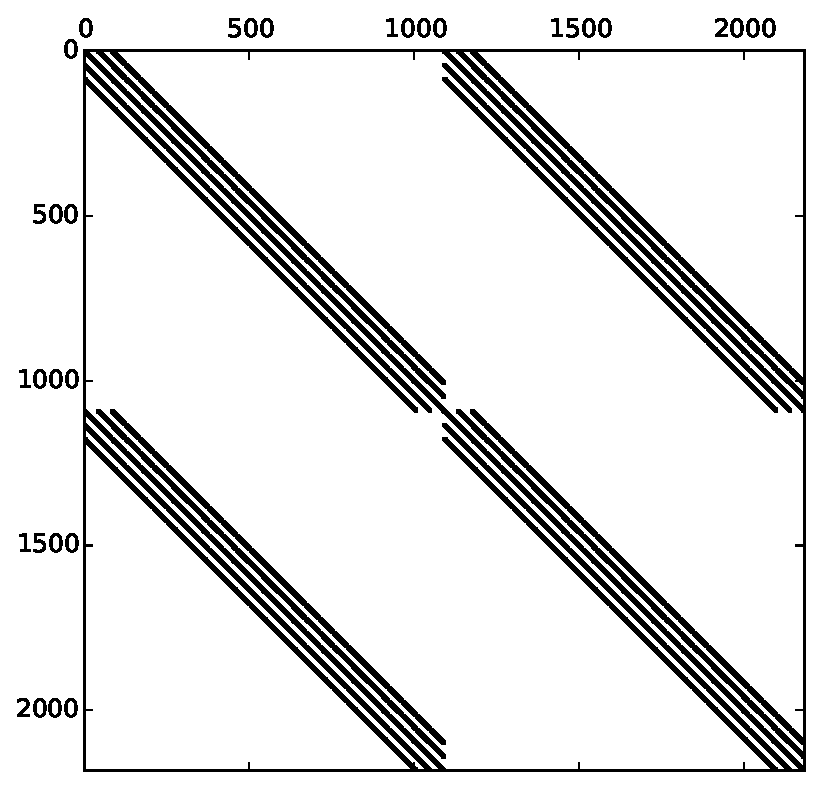
\includegraphics[width=0.49\columnwidth]{P_25_25-crop} \hfill
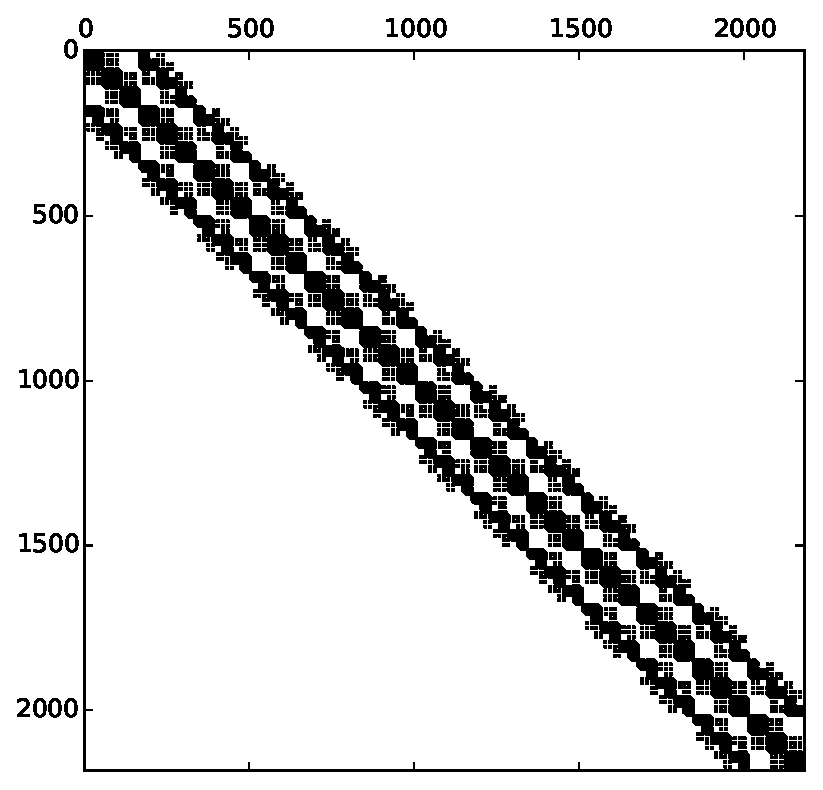
\includegraphics[width=0.49\columnwidth]{P_25_25_perm-crop}
\caption{A \texttt{spy} plot of $\mathcal{P}(\tau)$ for the \texttt{wedge} problem (left) and $\Psi^\mathsf{T} \mathcal{P}(\tau) \Psi$ (right) for $d=p=2$, and \texttt{nnz=100,587} in both cases. Clearly, the permutation leads to a reduction in bandwidth, and the permuted matrix is block tri-diagonal.}
\label{fig:perm}
\end{figure}

If the matrix \eqref{eq:L2Msss} is sparse, it is advisable to use a sparse data structure on generator-level for \eqref{P11}-\eqref{P22} as well. Because of Corollary \ref{tri_perm}, the permuted 2D preconditioner can be written as,
\begin{equation}
\label{eq:perm_precon}
         \mathcal{P}_{2D}= \Psi^\mathsf{T} \mathcal{P}(\tau) \Psi =\begin{bmatrix}
                     P_{1,1} & P_{1,2} &         &        \\
                     P_{2,1} & P_{2,2} & P_{2,3} &        \\
%                              & P_{3,2} & P_{3,3} & \ddots & \\
                                     & \ddots  & \ddots & \ddots \\
                                     &         & \ddots & P_{n_x, n_x}
                 \end{bmatrix}
\end{equation}
with block entries $P_{i,j}$ in SSS format according to \mbox{Definition \ref{def_sss}}, compare Figure \ref{fig:perm} (right). We perform a block-LU factorization of the form $\mathcal{P}_{2D} = L S U$, with 
\begin{equation}
\label{eq:full_Schur}
        L_{i,j}=\begin{cases}
             I &\hspace{-0.2cm} \text{if}\ i=j \\
             P_{i,j}S_j^{-1} &\hspace{-0.2cm} \text{if}\ i = j+1
	     \end{cases}, \
	U_{i,j}=\begin{cases}
             I &\hspace{-0.2cm} \text{if}\ j=i \\
             S_i^{-1}P_{i,j} &\hspace{-0.2cm} \text{if}\ j = i+1
	     \end{cases},     
\end{equation}
and Schur complements given by
\begin{equation}\label{eqn_schur}
        S_i=\begin{cases}
             P_{i,i} & \text{if}\ i=1 \\
             P_{i,i}-P_{i,i-1}S_{i-1}^{-1}P_{i-1,i} & \text{if}\ 2\leq i\leq n_x.
	     \end{cases}
\end{equation}

The Schur complements in \eqref{eq:full_Schur}-\eqref{eqn_schur} are SSS matrices and inverses can be computed with Algorithm \ref{LU}. From Lem\-ma \ref{lu_sss}, we conclude that this does not increase the respective off-diagonal ranks. However, in \eqref{eq:full_Schur}-\eqref{eqn_schur}, we also need to perform matrix-matrix multiplications and additions of SSS matrices which lead to an increase in rank, cf. \cite{CD05} and Appendix \ref{app_matmulsss}. Therefore, we apply model order reduction in the sense of Definition \ref{mor_sss} at each step $i$ of the recursion \eqref{eqn_schur} in order to limit the off-diagonal rank. An algorithm that limits the off-diagonal ranks to a constant, say $r^\ast$, can be found in \cite{QG15}. This leads to approximate Schur complements and, hence, an inexact $LU$ factorization. In Experiment \ref{exp:off_rank}, we show that for small off-diagonal ranks this approach results in a very good preconditioner for 2D elastic problems.

\subsection{SSOR splitting using MSSS computations for 3D problems}
\label{ch_msss3d}
For 3D problems, we consider a nodal-based FEM discretization of \eqref{eq:precon} with $n_z$ being the outermost dimension, as shown in Figure \ref{fig:precon3d} for different order of B-splines. In order to derive a memory-efficient algorithm for 3D problems, we consider the matrix splitting,
\begin{align}
\label{eq:splitting}
\mathcal{P}_{3D}(\tau) = \underbar{L} + \hat{S} + \overbar{U}, \quad \hat{S} = \text{blkdiag}(\hat{S}_1,...,\hat{S}_{n_z}),
\end{align}
where $\underbar{L}$ and $\overbar{U}$ are the (sparse) strictly lower and strictly upper parts of $\mathcal{P}_{3D}(\tau)$, and $\hat{S}$ is a block-diagonal matrix with blocks $\hat{S}_i$ being in level-2 MSSS structure. This data structure is illustrated in Figure \ref{L3scheme}.

 \begin{figure}[ht]
     \centering
     \begin{subfigure}{0.31\columnwidth}
         \centering
         \includegraphics[width=\textwidth]{P3d_p1-crop_small.pdf}%{figs/P3d_p1-crop.pdf}
         \caption{$p=1$}
     \end{subfigure}%
     ~ 
     \begin{subfigure}{0.31\columnwidth}
         \centering
         \includegraphics[width=\textwidth]{P3d_p2-crop_small.pdf}%{figs/P3d_p2-crop.pdf}
         \caption{$p=2$}
     \end{subfigure}
     ~ 
     \begin{subfigure}{0.31\columnwidth}
         \centering
 	\includegraphics[width=\textwidth]{P3d_p3-crop_small.pdf}%{figs/P3d_p3-crop.pdf}
         \caption{$p=3$}
     \end{subfigure}
     \caption{Nodal-based discretization of $\mathcal{P}_{3D}(\tau)$ in 3D for different degrees $p$ of FEM basis function.} \label{fig:precon3d}
 \end{figure}
According to \cite[Section 4.1.2]{S03}, the SSOR preconditioner based on the splitting \eqref{eq:splitting} is given by,
\begin{align*}
\mathcal{P}_{3D}(\tau) = \frac{1}{\ssorfac(2-\ssorfac)}(\ssorfac\ \underbar{L}+\hat{S}) \hat{S}^{-1} (\ssorfac\ \overbar{U}+\hat{S})
\end{align*}
which for $\ssorfac=1$ equals,
\begin{align}
\label{eq:approx_Schur}
\mathcal{P}_{3D}(\tau) = (\underbar{L}\hat{S}^{-1} + I) \hat{S} (\hat{S}^{-1}\overbar{U} + I).
\end{align}
In \eqref{eq:approx_Schur} we note that this decomposition coincides with the 2D approach \eqref{eq:full_Schur}-\eqref{eqn_schur} when the term ``$P_{i,i-1}S_{i-1}^{-1}P_{i-1,i}$'' in the Schur complements \eqref{eqn_schur} is neglected. This choice avoids a rank increase due to multiplication and addition, but yields a \textit{worse} preconditioner than in 2D. The block entries $\hat{S}_i$ ,$i=1,..,n_z$, are in level-2 MSSS structure and, hence, formula \eqref{eq:full_Schur}-\eqref{eqn_schur} can be applied sequentially for the inverses that appear in \eqref{eq:approx_Schur}. In order to invert level-1 SSS matrices that recursively appear in \eqref{eqn_schur}, we use Algorithm \ref{LU}. On the generator level, we use suitable \texttt{LAPACK} routines; cf. Table \ref{tab:algorithms} for an overview of the different algorithms used at each level.
\begin{table}[H]
\centering
\caption{Overview of algorithms applied at different levels for the (approximate) inversion of the preconditioner \eqref{eq:approx_Schur}.}\label{tab:algorithms}
\begin{tabular}{|c|c|c|}
 \hline
 \textbf{level} & \textbf{algorithm for} $\mathbf{(\cdot)^{-1}}$& \textbf{datatype} \\
 \hline
 3D MSSS& SSOR decomposition \eqref{eq:approx_Schur} & \texttt{sparse} + \texttt{L2\_SSS}\\
 2D MSSS & Schur \eqref{eq:full_Schur}-\eqref{eqn_schur} \& MOR & \texttt{tridiag. L2\_SSS} \\
 1D SSS\phantom{M}& Algorithm \ref{LU} & \texttt{L1\_SSS} \eqref{eqn_sss_definition}\\
 generator & \texttt{LAPACK} routines & set of sparse matrices\\
 \hline
\end{tabular}
\end{table}

We illustrate the data structure of the preconditioner \eqref{eq:approx_Schur} in 3D for the case of linear B-splines ($p=1$) in Figure \ref{fig:datastruc}. On level-3, we use a mixed data format that is most memory-efficient for the splitting \eqref{eq:splitting}. Since only diagonal blocks need to be inverted, we convert those to level-2 MSSS format, and keep the off-diagonal blocks of $\underbar{L}$ and $\overbar{U}$ in sparse format.
\begin{figure}[ht]
    \centering
    \begin{subfigure}{0.3\columnwidth}
        \centering
        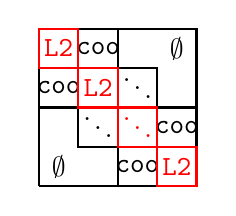
\begin{tikzpicture}
              
          \draw[black,thick] (0.5,2) -- (0.5,1.5) --(1,1.5) -- (1,2) -- (0.5,2);
          \node at (0.75,1.75) {\color{black}{\texttt{coo}}};
          
          \draw[black,thick] (0,1.5) -- (0,1) --(0.5,1) -- (0.5,1.5) -- (0,1.5);
          \node at (0.25,1.25) {\color{black}{\texttt{coo}}};
          
           \draw[black,thick] (0.5,1) -- (0.5,0.5) --(1,0.5) -- (1,1) -- (0.5,1);
           \node at (0.75,0.85) {\color{black}{$\ddots$}};
          
           \draw[black,thick] (1,0.5) -- (1,0) --(1.5,0) -- (1.5,0.5) -- (1,0.5);
           \node at (1.25,0.25) {\color{black}{\texttt{coo}}};
           
           \draw[black,thick] (1,1.5) -- (1,1) --(1.5,1) -- (1.5,1.5) -- (1,1.5);
           \node at (1.25,1.35) {\color{black}{$\ddots$}};
           
           \draw[black,thick] (1.5,1) -- (1.5,0.5) --(2,0.5) -- (2,1) -- (1.5,1);
           \node at (1.75,0.75) {\color{black}{\texttt{coo}}};

           
           \draw[thick] (0,0) -- (2,0) -- (2,2) -- (0,2) -- (0,0);
          
           
          \draw[red,thick] (0,2) -- (0,1.5) --(0.5,1.5) -- (0.5,2.0) -- cycle;
          \node at (0.25,1.75) {\color{red}{\texttt{L2}}};
          
          \draw[red,thick] (0.5,1.5) -- (0.5,1) --(1,1) -- (1,1.5) -- (0.5,1.5);
          \node at (0.75,1.25) {\color{red}{\texttt{L2}}};
          
          \draw[red,thick] (1,1) -- (1,0.5) --(1.5,0.5) -- (1.5,1) -- (1,1);
          \node at (1.25,0.85) {$\color{red}{\ddots}$};

          \draw[red,thick] (1.5,0.5) -- (1.5,0) --(2,0) -- (2,0.5) -- (1.5,0.5);
          \node at (1.75,0.25) {\color{red}{\texttt{L2}}};
          
          \node at (0.25,0.25) {$\emptyset$};
          \node at (1.75,1.75) {$\emptyset$};
          
          
%           \draw[red,thick,overlay,->] (0.25,2) to [bend left=35] (2.75,2);
          
        \end{tikzpicture}
        \caption{\texttt{L3\_SSS}}\label{L3scheme}
    \end{subfigure}%
    ~ 
    \begin{subfigure}{0.3\columnwidth}
        \centering
         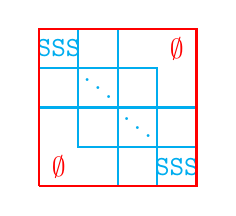
\begin{tikzpicture} 
                   
          \draw[cyan,thick] (0,2) -- (0,1.5) --(0.5,1.5) -- (0.5,2.0) -- (0,2);
          \node at (0.25,1.75) {\color{cyan}{\texttt{SSS}}};
          
          \draw[cyan,thick] (0.5,1.5) -- (0.5,1) --(1,1) -- (1,1.5) -- (0.5,1.5);
          \node at (0.75,1.35) {$\color{cyan}{\ddots}$};
          
          \draw[cyan,thick] (1,1) -- (1,0.5) --(1.5,0.5) -- (1.5,1) -- (1,1);
          \node at (1.25,0.85) {$\color{cyan}{\ddots}$};

          \draw[cyan,thick] (1.5,0.5) -- (1.5,0) --(2,0) -- (2,0.5) -- (1.5,0.5);
          \node at (1.75,0.25) {\color{cyan}{\texttt{SSS}}};
                   
          
          \draw[cyan,thick] (0.5,2) -- (0.5,1.5) --(1,1.5) -- (1,2) -- (0.5,2);
%           \node at (0.75,1.75) {\color{cyan}{\texttt{SSS}}};
          
          \draw[cyan,thick] (0,1.5) -- (0,1) --(0.5,1) -- (0.5,1.5) -- (0,1.5);
%           \node at (0.25,1.25) {\color{cyan}{\texttt{SSS}}};
          
          \draw[cyan,thick] (0.5,1) -- (0.5,0.5) --(1,0.5) -- (1,1) -- (0.5,1);
%           \node at (0.25,1.25) {\color{cyan}{\texttt{SSS}}};
          
           \draw[cyan,thick] (1,0.5) -- (1,0) --(1.5,0) -- (1.5,0.5) -- (1,0.5);
%           \node at (0.25,1.25) {\color{cyan}{\texttt{SSS}}};

           \draw[cyan,thick] (1,1.5) -- (1,1) --(1.5,1) -- (1.5,1.5) -- (1,1.5);
%           \node at (0.25,1.25) {\color{cyan}{\texttt{SSS}}};

           \draw[cyan,thick] (1.5,1) -- (1.5,0.5) --(2,0.5) -- (2,1) -- (1.5,1);
%           \node at (0.25,1.25) {\color{cyan}{\texttt{SSS}}};
          
          
          \node at (0.25,0.25) {$\color{red}{\emptyset}$};
          \node at (1.75,1.75) {$\color{red}{\emptyset}$};
          
          \draw[red, thick] (0,0) -- (2,0) -- (2,2) -- (0,2) -- (0,0);
        \end{tikzpicture}
        \caption{\texttt{L2\_SSS}, def. \ref{def_msss}}\label{L2scheme}
    \end{subfigure}
    ~ 
    \begin{subfigure}{0.3\columnwidth}
        \centering
         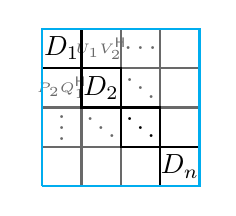
\begin{tikzpicture}
          
          \draw[dimgray,thick] (0.5,2) -- (0.5,1.5) --(1,1.5) -- (1,2) -- (0.5,2);
          \node at (0.75,1.75) {\tiny{$\color{dimgray}{U_1 V_2^\trp}$}};
          
           \draw[dimgray,thick] (1,1.5) -- (1,1) --(1.5,1) -- (1.5,1.5) -- (1,1.5);      
           \node at (1.25,1.35) {$\color{dimgray}{\ddots}$};
           
           \draw[dimgray,thick] (1.5,1) -- (1.5,0.5) --(2,0.5) -- (2,1) -- (1.5,1);
%            \node at (1.75,0.85) {$\color{dimgray}{\ddots}$};
           
           \draw[dimgray,thick] (1,0.5) -- (1,0) --(1.5,0) -- (1.5,0.5) -- (1,0.5);
%            \node at (1.25,0.35)  {$\color{dimgray}{\ddots}$};
           
           \draw[dimgray,thick] (0,1.5) -- (0,1) --(0.5,1) -- (0.5,1.5) -- (0,1.5);
          \node at (0.25,1.25) {\tiny{$\color{dimgray}{P_2 Q_1^\trp}$}};
          
           \draw[dimgray,thick] (0.5,1) -- (0.5,0.5) --(1,0.5) -- (1,1) -- (0.5,1);
           \node at (0.75,0.85) {\color{dimgray}{$\ddots$}};
          
           \draw[dimgray,thick] (0,0.5) -- (0.5,0.5);
           \draw[dimgray,thick] (0.5,0.5) -- (0.5,0);
           
           \draw[dimgray,thick] (1.5,2) -- (1.5,1.5);
           \draw[dimgray,thick] (1.5,1.5) -- (2,1.5);
           
           \node at (1.25,1.75) {$\color{dimgray}{\hdots}$};
           \node at (0.25,0.85) {$\color{dimgray}{\vdots}$};
           
          
          \draw[black,thick] (0,2) -- (0,1.5) --(0.5,1.5) -- (0.5,2.0) -- (0,2);
          \node at (0.25,1.75) {$\color{black}{D_1}$};
          
          \draw[black,thick] (0.5,1.5) -- (0.5,1) --(1,1) -- (1,1.5) -- (0.5,1.5);
          \node at (0.75,1.25) {$\color{black}{D_2}$};
          
          \draw[black,thick] (1,1) -- (1,0.5) --(1.5,0.5) -- (1.5,1) -- (1,1);
          \node at (1.25,0.85) {$\color{black}{\ddots}$};

          \draw[black,thick] (1.5,0.5) -- (1.5,0) --(2,0) -- (2,0.5) -- (1.5,0.5);
          \node at (1.75,0.25) {$\color{black}{D_n}$};
          
          
          \draw[cyan, thick] (0,0) -- (2,0) -- (2,2) -- (0,2) -- (0,0);
    
          
        \end{tikzpicture}
        \caption{\texttt{SSS}, def. \ref{def_sss}}\label{L1scheme}
    \end{subfigure}
    \caption{Nested data structure for the preconditioner \eqref{eq:perm_precon} after permutation for $d=3$ and $p = 1$. With \texttt{'coo'} we abbreviate the coordinate-based sparse data structure as used, for instance, in \cite{sparsekit}.}\label{fig:datastruc}
\end{figure}

For $p>1$, we apply the permutation of Definition \ref{perm_msss} on each diagonal block of $\hat S$, cf. Figure \ref{fig:precon3d_level2}. This way, the Schur decomposition described in Section \ref{ch:msss_lu} can be applied for inverting block tri-diagonal level-2 MSSS matrices.
\begin{figure}[ht]
    \centering
    \begin{subfigure}{0.45\columnwidth}
        \centering
        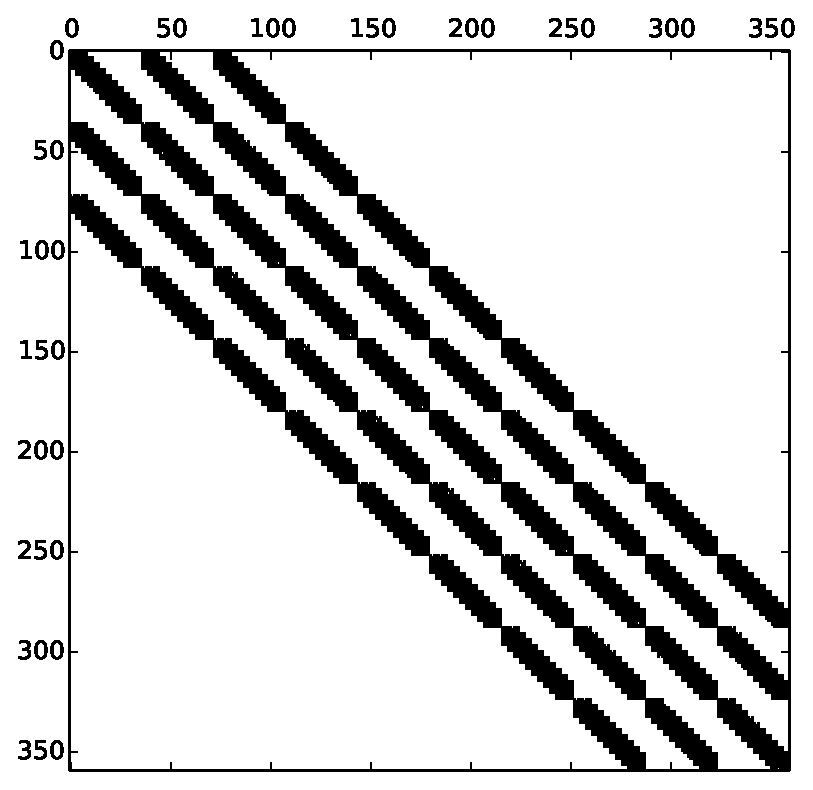
\includegraphics[width=\textwidth]{Si_p2-crop}
        \caption{$\hat{S}_i, \ 1 \leq i \leq n_x$}
    \end{subfigure}%
    ~ \hfill
    \begin{subfigure}{0.45\columnwidth}
        \centering
        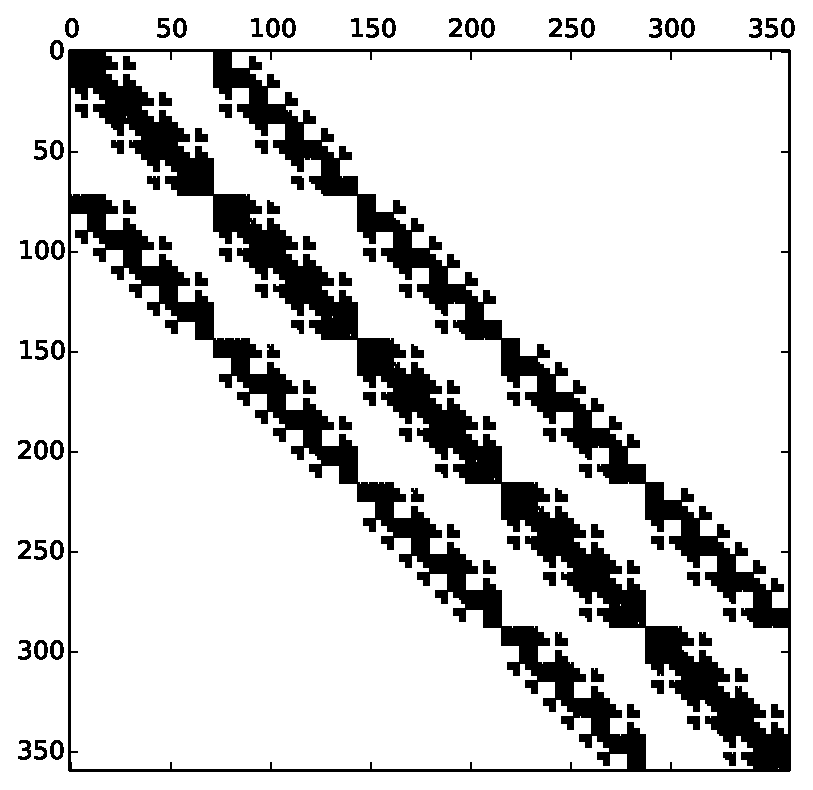
\includegraphics[width=\textwidth]{Si_p2_perm-crop}
        \caption{$\Psi^\mathsf{T} \hat{S}_i \Psi$}
    \end{subfigure}

    \caption{Permutation on level-2 leads to a block tri-diagonal level-2 MSSS matrix for $p>1$.} \label{fig:precon3d_level2}
\end{figure}

\subsection{Memory analysis for 2D and 3D MSSS preconditioner}
We finish our description of MSSS preconditioners with a memory analysis of the suggested algorithms described for 2D problems in Section \ref{ch:msss_lu}, and for 3D problems in Section \ref{ch_msss3d}, respectively. The following Corollary \ref{mem_3d} shows that in both cases we obtain linear memory requirements in terms of the problem size \eqref{eq:unknows}.
\begin{figure}[ht]
    \centering
    \begin{tikzpicture}
     \node at (0,0) {\includegraphics[scale=0.2]{z_planes2.png}};
     \node at (-1.3,1.3)  {${\color{white}\mathbf{\hat{S}_1}}$};
     \node at (-1.18,0.7)  {${\color{white}\mathbf{\hat{S}_2}}$};
     \node at (-1.01,0.04) {${\color{white}\mathbf{\hat{S}_3}}$};
     
     \node at (-0.6,-1.65) {${\color{white}\mathbf{\hat{S}_{n_z}}}$};
     
     \draw [->] (-2.4,1.0) -- (-2.15,-0.1);
     \node at (-2.55,0.7) {$z$};
    \end{tikzpicture}
    \caption{Schematic illustration: The diagonal blocks of $\hat{S}$ in \eqref{eq:splitting} correspond to a sequence of $n_z$ 2D problems in the $xy-$plane.} \label{fig:3dscheme}
\end{figure}
\begin{corollary}[Linear memory requirement]\label{mem_3d}
Consider \mbox{$p=1$} and a three-dimensional problem of size $n_x \times n_y \times n_z$. For simplicity, we assume on the generator-level $m_i \equiv m$, and the off-diagonal ranks of the inverse Schur complements $S_i$ in \eqref{eqn_schur} being limited by $k_i = l_i\equiv r^\ast$. The grid size in $y$-direction on level-1 implies $n$ generators via $n = d n_y m^{-1}$, with $m$ being a constant and $d \in \{2,3\}$. The memory requirement of the preconditioners $\mathcal{P}_{2D}$ and $\mathcal{P}_{3D}$ presented in Section \ref{ch:msss_lu} and Section \ref{ch_msss3d}, respectively, is linear in the respective problem dimension \eqref{eq:unknows}.
\end{corollary}
\begin{proof}
Consider the preconditioner $\mathcal{P}_{2D}=LSU$ given by \eqref{eq:full_Schur}-\eqref{eqn_schur}. Besides blocks of the original operator, an additional storage of $n_x$ inverse Schur complements $S_i^{-1}$ in SSS format is required,
\begin{align*}
 \texttt{mem}(\mathcal{P}_{2D}^{-1},r^\ast) &= \texttt{mem}(\mathcal{P}_{2D})  + \sum_{i=1}^{n_x} \texttt{mem}(S_{i}^{-1},r^\ast) \in \mathcal{O}(n_xn_y).
\end{align*}
The approximate Schur decomposition described in Section \ref{ch:msss_lu} allows dense, full rank diagonal generators $D_i, 1 \leq i \leq n,$ of size $m \times m$, and limits the rank of all off-diagonal generators by $r^\ast$ using model order reduction techniques:
\begin{align*}
\texttt{mem}(S_{i}^{-1},r^\ast) = \underbrace{n \cdot m^2}_{\sim D_i} + \underbrace{4(n-1)mr^\ast}_{\sim \{U_i,V_i,P_i,Q_i\}} + \underbrace{2(n-2)r^\ast r^\ast}_{\sim \{W_i,R_i\}} \in \mathcal{O}(n_y).
\end{align*}
Concerning the memory requirement for storing $\mathcal{P}_{2D}$ in MSSS format, we first note that the permutation described in Corollary \ref{tri_perm} does not affect the memory consumption. Since we use sparse generators in \eqref{P11}-\eqref{P22}, the memory requirement is of the same order as the original, sparse matrix \eqref{eq:precon} obtained from the FEM discretization.

For 3D problems, we suggest the usage of $\mathcal{P}_{3D}$ as in \eqref{eq:approx_Schur} based on the splitting \eqref{eq:splitting}. For the data structure, we keep the strictly lower and upper diagonal parts in sparse format and convert the diagonal blocks to level-2 MSSS format, cf. Figure \ref{fig:3dscheme},
\begin{align*}
 \texttt{mem}(\mathcal{P}_{3D}^{-1},r^\ast) &=  n_z \cdot \texttt{mem}(\mathcal{P}_{2D}^{-1},r^\ast) + \texttt{nnz}(\underbar{L}) + \texttt{nnz}(\overbar{U}) \\ &\in \mathcal{O}(n_xn_yn_z).
\end{align*}
\qed
\end{proof}
Note that the case $p>1$ also yields a linear memory requirement but is, for simplicity, not addressed here.

\section{Numerical experiments}
\label{ch:num}
We present numerical examples\footnote{All test cases are publicly available from the author's \href{https://github.com/ManuelMBaumann/elastic_benchmarks}{github} repository \cite{Bgithub}.} for the two-dimensional, elastic \marmousi model \cite{marm2} as well as for a three-di\-men\-sional elastic \texttt{wedge} problem which has been inspired by the well-known acoustic test case introduced in \cite{Knibbe2016,PM04} for 2D and 3D, respectively. In the examples, we restrict ourselves to Cartesian grids with fixed discretization size \mbox{$h \equiv h_x = h_y = h_z$}. Depending on the specific problem parameters, the maximum frequency we allow is restricted by,
\begin{align*}
f_\text{max} < \frac{\text{min}_{\mathbf{x} \in \Omega}\{c_p,c_s\}}{ppw \cdot h}, \quad ppw = 20,
%  ppw = \frac{\lambda_{\text{min}}}{h}, \quad \text{with } \lambda_{\text{min}} = \frac{\text{min}\{c_{p,s}(\mathbf{x})\}}{f_\text{max}}
\end{align*}
where in the following experiments a minimum of $20$ points per wavelength ($ppw$) is guaranteed, and $\omega_k = 2 \pi f_k$.

All numerical examples presented in this section have been implemented in FORTRAN 90
using the GNU/gfortran compiler running over GNU/Debian Linux, and executed on a computer with 
4 CPUs Intel I5 with 32 GB of RAM.
\subsection{Parameter studies}
 We begin our numerical tests with a sequence of experiments performed on an \textit{academic} two-dimensional \texttt{wedge} problem described in Figure \ref{fig:wedge2d}. The aim of these first experiments is to prove the following concepts for the 2D algorithm introduced in Section \ref{ch:msss_lu}:
 \begin{itemize}
  \item Demonstrate the dependency of the iterative solution meth\-od on the maximum off-di\-ag\-o\-nal rank, $r^\ast = \max \{ r^l, r^u\}$. In Experiment \ref{exp:off_rank} we show that a small value of $r^\ast$ leads to a very good preconditioner in terms of number of Krylov iterations.
  \item Show that the 2D algorithm yields linear computational complexity when all problem parameters are unchanged and the grid size doubles (Experiment \ref{exp:lin_compl}).
  \item In Experiments \ref{exp:freq1} and \ref{exp:freq2}, we evaluate the frequency dependency of the MSSS-preconditioner \eqref{eq:precon} when $\tau \neq \omega$. This is in particular important when multiple frequencies in a matrix equation framework are considered in Section \ref{ch:best_tau}.
 \end{itemize}
 
\begin{figure}[H]
  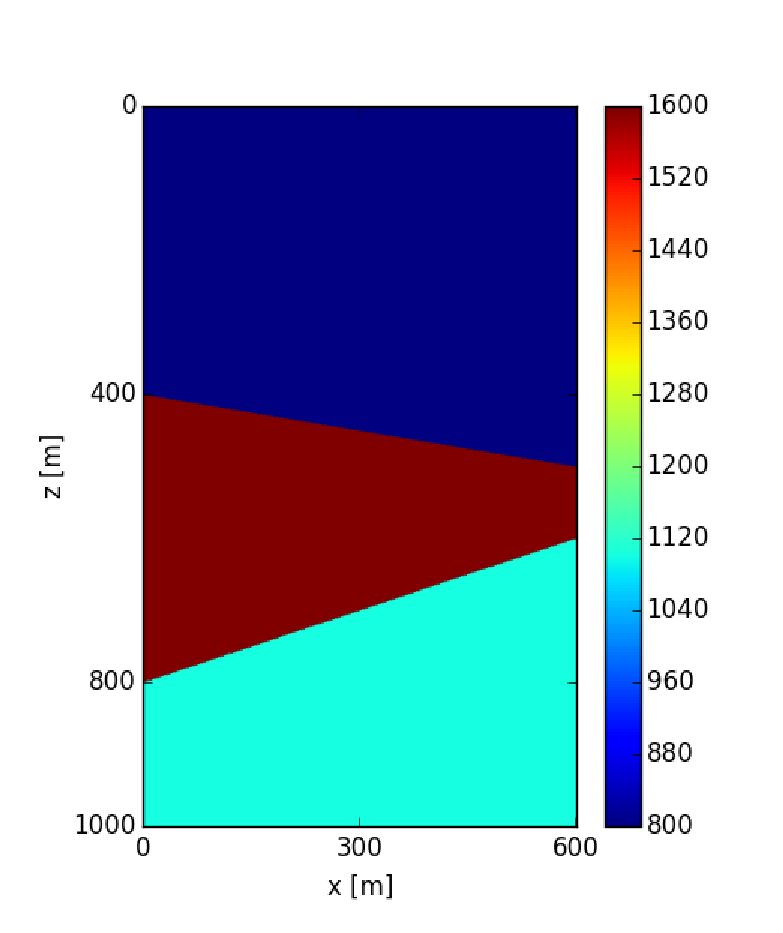
\includegraphics[width=0.49\columnwidth]{wedge2d_cs} \hfill
  \includegraphics[width=0.49\columnwidth]{wedge2d_uz}
\caption{2D elastic \texttt{wedge} problem used for parameter study: Speed of S-waves in $m/s$ (left) and real part of $z$-component of displacement vector at $f = 16$ Hz (right).}
\label{fig:wedge2d}
\end{figure}

We perform parameter studies on a two-dimensional slice ($xz$-plane) of the \texttt{wedge} problem described in Figure \ref{fig:wedge3d_par}. The values of $\rho, c_p$ and $c_s$ in the respective layers are given in Table \ref{tab_params}, and the considered computational domain $\Omega = [0,600] \times [0,1000]$ meters is shown in Figure \ref{fig:wedge2d}.

\begin{table}[ht]
\centering
 \caption{Parameter configuration of the elastic \texttt{wedge} problem. The Lam\'e parameters can be computed via \eqref{eq:lame}.} \label{tab_params} 
 \begin{tabular}{|l|c|c|c|}
 \hline
  Parameter & Layer \#1 & Layer \#2 & Layer \#3 \\
  \hline
  $\rho [kg/m^3]$ & 1800& 2100&1950 \\
  $c_p [m/s]$ & 2000&3000 & 2300\\
  $c_s [m/s]$ & \phantom{0}800&1600&1100 \\
  \hline
 \end{tabular}
\end{table}

% \subsubsection{Single-frequency case}
In the first set of experiments, we restrict ourselves to the single-frequency case, $\Nom = 1$. The discrete problem is, thus, given by,
\begin{align*}
 (K + i \omega C - \omega^2 M) \x = \rhs,
\end{align*}
with a preconditioner that approximates the original operator, $\mathcal{P}(\tau) \approx (K + i \tau C - \tau^2M),  \tau = \omega$, by taking low-rank approximations in the block-LU factorization.  

\begin{exper}[Off-diagonal rank] \label{exp:off_rank}
This experiment evaluates the performance of the MSSS-preconditioner \eqref{eq:perm_precon} for 2D problems when the maximal off-diagonal rank $r^\ast$ is in\-creased. 
\end{exper}
In Experiment \ref{exp:off_rank}, we apply the approximate block-LU decomposition \eqref{eq:full_Schur}-\eqref{eqn_schur} as described in Section \ref{ch:msss_lu} to the 2D \texttt{wedge} problem at frequencies $f=8$ Hz and $f=16$ Hz. The maximum off-diagonal rank $r^\ast = \max \{ r^l, r^u\}$ of the Schur complements \eqref{eqn_schur} is restricted using model order reduction techniques, cf. \cite{QG15}. The dimension of the diagonal constructors has been chosen to be $m_i = 40$, cf. Table \ref{tab_sss_size}. Figure~\ref{fig:exp1} shows the convergence behavior of preconditioned  IDR($4$) (Algorithm \ref{bio_idr} with $\Nom =1$) and preconditioned BiCGStab \cite{v92}. We note that even in the high-frequency case, an off-di\-ag\-o\-nal rank of $r^\ast = 10$ leads to a very efficient preconditioner, and an (outer) Krylov method that converges within at most $40$ iterations to a residual tolerance \texttt{tol=10e-8}. Moreover, we observe that IDR($s$) outperforms BiCGStab in the considered example when the same preconditioner is applied. For a rank $r^\ast > 15$, we observe convergence within very few iterations.
\begin{figure}[H]
  \includegraphics[width=\columnwidth]{order_2d_new.pdf}  
\caption{Number of Krylov iterations when the maximum off-diagonal rank of the inverse Schur complements is restricted to $r^\ast$.}
\label{fig:exp1}
\end{figure}

\begin{exper}[Computational complexity in 2D] \label{exp:lin_compl}
The inexact block-LU factorization yields linear computational complexity when applied as a preconditioner within MSSS-pre\-conditioned IDR($s$), demonstrated for the 2D wedge problem.
\end{exper}
In our second numerical experiment, the maximum off-di\-ag\-o\-nal rank is fixed to $r^\ast =15$ such that very few IDR iterations are required, and the computational costs in Figure \ref{fig:exp:linCompl} are dominated by the MSSS preconditioner. We solve the 2D \texttt{wedge} problem at frequency $8$ Hz for different mesh sizes and a finite element discretization with B-splines of degree $p = \{1,2\}$. In Figure \ref{fig:exp:linCompl}, the CPU time is recorded for different problem sizes: The mesh size $h$ is doubled in both spatial directions such that the number of unknowns quadruples according to \eqref{eq:unknows}. From our numerical experiments we see that the CPU time increases by a factor of $\sim 4$ for both, linear and quadratic, splines. This gives strong numerical evidence that the 2D MSSS computations are performed in linear computational complexity.

\begin{figure}[ht]
  \includegraphics[width=\columnwidth]{draw_fig_new2.pdf}
\caption{Linear computational complexity of preconditioned IDR($4$) for the 2D \texttt{wedge} problem at $f=8$ Hz.}
\label{fig:exp:linCompl}
\end{figure}

\begin{exper}[Constant points per wavelength] \label{exp:freq1}
Conver- gence behavior of MSSS-preconditioned IRD($s$) when the problem size and wave frequency are increased simultaneously.
\end{exper}
In the previous example, the wave frequency is kept constant while the problem size is increased which is of little practical use due to oversampling. We next increase the wave frequency \textit{and} the mesh size simultaneously such that a constant number of points per wavelength, $ppw=20$, is guaranteed.
\begin{table}[ht]
\centering
 \caption{Performance of the MSSS preconditioner when problem size and frequency are increased simultaneously such that $ppw = 20$ and \texttt{tol=10e-8}: $\mathcal{O}(n^3)$ complexity.} \label{tab_freq_indep} 
 \begin{tabular}{|c|c|c|c|c|c|}
 \hline
  $f$ & $h [m]$ & $r^\ast$ & MSSS & IDR($4$) & total CPU time\\
  \hline
  $\phantom{0}4$ Hz & $10.0$& \phantom{0}5& 0.55 sec& \phantom{0}16 iter.& \phantom{0}0.71 sec\\
  $\phantom{0}8$ Hz & $\phantom{0}5.0$& \phantom{0}7 & 2.91 sec& \phantom{0}33 iter.& \phantom{00}4.2 sec \\
  $16$ Hz & $\phantom{0}2.5$& 10 &  15.3 sec& \phantom{0}62 iter.& \phantom{0}31.8 sec\\
  $32$ Hz & $1.25$& 16& 95.4 sec&101 iter. & 242.5 sec\\
  \hline
 \end{tabular}
\end{table}
In Table \ref{tab_freq_indep}, we use the freedom in choosing the maximum off-diagonal rank parameter $r^\ast$ such that the overall preconditioned IDR($s$) algorithm converges within a total number of iterations that grows linearly with the frequency.  This particular choice of $r^\ast$ shows that the MSSS preconditioner has comparable performance to the multi-grid approaches in \cite{Plessix2007,Rizzuti2016} where the authors numerically prove $\mathcal{O}(n^3)$ complexity for 2D problems of size $n_x = n_y \equiv n$.

The off-diagonal rank parameter $r^\ast$ can on the other hand be used to tune the preconditioner in such a way that the number of IDR iterations is kept constant for various problem sizes. In Table \ref{tab_freq_indep2}, we show that a constant number of $\sim 30$ IDR iterations can be achieved by a moderate increase of $r^\ast$ which yields an algorithm that is nearly linear.
\begin{table}[ht]
\centering
 \caption{Performance of the MSSS preconditioner when problem size and frequency are increased simultaneously such that $ppw = 20$ and \texttt{tol=10e-8}: Constant number of iterations.} \label{tab_freq_indep2}
 \begin{tabular}{|c|c|c|c|c|c|}
 \hline
  $f$ & $h [m]$ & $r^\ast$ & MSSS & IDR($4$) & total CPU time\\
  \hline
  $\phantom{0}4$ Hz & $10.0$& \phantom{0}3 & \phantom{0}0.50 sec & 29 iter.& \phantom{0}0.83 sec\\
  $\phantom{0}8$ Hz & $\phantom{0}5.0$& \phantom{0}7 &  \phantom{0}2.91 sec & 33 iter.& \phantom{00}4.2 sec \\
  $16$ Hz & $\phantom{0}2.5$& 11 & \phantom{0}16.9 sec& 27 iter.& \phantom{0}24.5 sec\\
  $32$ Hz & $1.25$& 18& 107.1 sec & 33 iter. & 163.2 sec\\
  \hline
 \end{tabular}
\end{table}

\begin{exper}[Quality of $\mathcal{P}_{2D}(\tau)$ when $\tau \neq \omega$] \label{exp:freq2}
Single-fre- quency experiments when seed frequency differs from the original problem. 
\end{exper}

\begin{figure}[H]
  \includegraphics[width=\columnwidth]{iter_vs_tau_new.pdf}  
\caption{Number of iterations of preconditioned IDR($s$) when $\tau \neq \omega$ in \eqref{eq:perm_precon}. We perform the experiment for different frequencies, and keep a constant grid size $h=5m$ and residual tolerance \texttt{tol = 10e-8}.}
\label{fig:iter_vs_tau}
\end{figure}

This experiments bridges to the multi-frequency case. We consider single-frequency problems at $f \in \{2,3,4,5\}$~Hz, and vary the parameter $\tau$ of the preconditioner \eqref{eq:perm_precon}. The off-diagonal rank $r^\ast$ is chosen sufficiently large such that fast convergence is obtained when $\tau = \omega$. From Figure \ref{fig:iter_vs_tau} we conclude that the quality of the preconditioner heavily relies on the seed frequency, and a fast convergence of preconditioned IDR($4$) is only guaranteed when $\tau$ is close to the original frequency.

% \subsubsection{Multi-frequency case}
\subsection{The elastic \marmousi model}
\label{ch:best_tau} 
We now consider the case when $\Nom > 1$, and the matrix equation,
\begin{align}
\label{eq:me2}
K \X + i C \X \Sigma - M \X \Sigma^2 = \blkrhs, \quad \X \in \mathbb{C}^{\n \times \Nom},
\end{align}
is solved. Note that this way we can incorporate multiple wave frequencies in the diagonal matrix $\Sigma = \text{diag}(\omega_1,...,\omega_\Nom)$, and different source terms lead to a block right-hand side of the form $\blkrhs = [\rhs_1,...,\rhs_\Nom]$. When multiple frequencies are present, the choice of seed frequency $\tau$ is crucial as we demonstrate for the \marmousi problem in Experiment~\ref{multifreq}.
% \subsection{The elastic \marmousi model}
We solve the matrix equation \eqref{eq:me2} arising from the realistic \marmousi problem \cite{marm2}. We consider a subset of the computational domain, $\Omega = [0,4000] \times [0,1850] m$, as suggested in \cite{Rizzuti2016}, cf. Figure \ref{fig:marm}.

\begin{exper}[\marmousi at multiple right-hand sides]\label{multiRHS}
Per\-for\-mance of the MSSS-preconditioned IDR(s) method for the two-dimensional \marmousi problem when multiple source locations are present.
\end{exper}
We consider the \marmousi problem depicted in Figure~\ref{fig:marm} at $h=5$m and frequency $f=2$ Hz. We present the performance of MSSS-preconditioned IDR($4$) for $\Nom$ e\-qually-spaced source locations (right-hand sides) in Table \ref{tab_mar2}. The CPU time required for the preconditioner as well as the iteration count is constant when $\Nom > 1$ because we consider a single frequency. The overall wall clock time, however, scales better than $\Nom$ due to the efficient implementation of block matrix-vector products in the IDR algorithm. The experiment for $\Nom=20$ shows that there is an optimal number of right-hand sides for a single-core algorithm.

 \begin{table}[H]
 \caption{Numerical experiments for the \marmousi problem at $f=2$ Hz using a maximum off-diagonal rank of $r^\ast=15$.} \label{tab_mar2}
  \centering
  \begin{tabular}{|c|c|c|}
  \hline
   \# RHSs & MSSS fact. [sec] & IDR(4) [sec]\\
   \hline
   1 & 60.2 & \phantom{0}8.18  (8 iter.) \\
   5 & 60.2 & \phantom{0}25.0 (8 iter.) \\
   10 & 60.1  &\phantom{0}43.5 (8 iter.)\\
   20 & 60.3 &  108.3 (8 iter.) \\
   \hline
  \end{tabular}
 \end{table}

\begin{figure}[H]
  \includegraphics[width=0.98\columnwidth]{cs-crop.eps}\\
  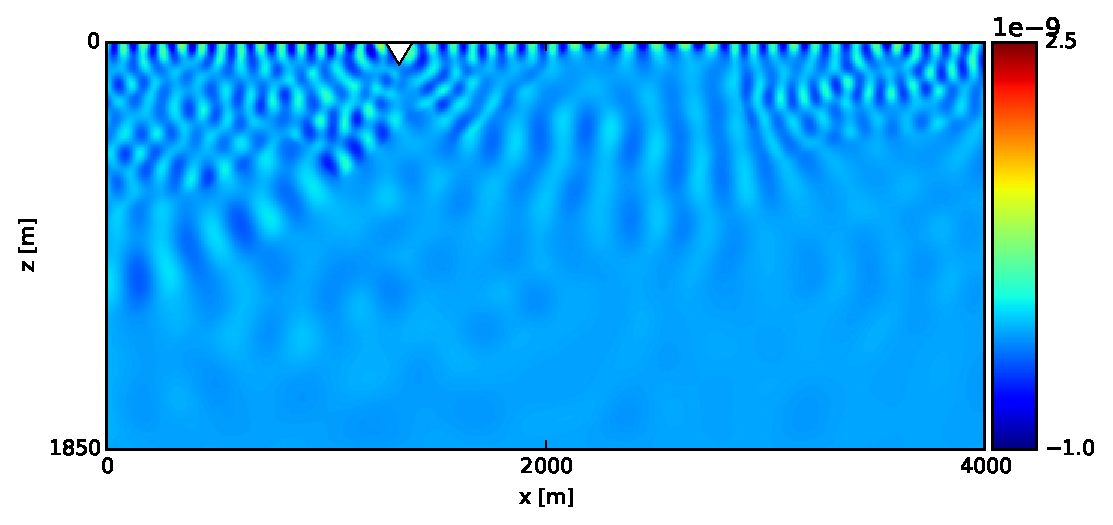
\includegraphics[width=0.98\columnwidth]{disp_z10_f4-crop.eps}\\
  \includegraphics[width=0.98\columnwidth]{disp_z10_f6-crop.eps}

\caption{Speed of S-waves in $m/s$ (top), and real part of the $z$-component of the displacement vector in frequency-domain at $f=4$ Hz (middle) and $f=6$ Hz (bottom) for the \marmousi model, cf. \cite{marm2} for a complete parameter set. The source location is indicated by the symbol '$\triangledown$'.}
\label{fig:marm}
\end{figure}

\begin{exper}[\marmousi at multiple frequencies]\label{multifreq}
Per\-for\-mance of MSSS-preconditioned IDR(s) for the two-di\-men\-sional \marmousi problem at multiple frequencies.
\end{exper}

 \begin{figure}[H]
 \centering
  \includegraphics[width=0.6\columnwidth]{ms_time.pdf}
%   \includegraphics[width=0.6\columnwidth]{ms_rot_new.pdf}
  \caption{Total CPU times of MSSS-IDR($4$) for $\Nom > 1$ frequencies equally-spaced within a fixed range. Additional scaling (dashed lines) following \cite{BvG17} improves convergence, and allows for larger frequency ranges.}\label{fig:multiF}
 \end{figure}
 In Experiment \ref{multifreq}, we consider a single source term located at $(L_x/2,0)^\mathsf{T}$ and $\Nom$ frequencies equally-spaced in the intervals $f_k \in [2.4,2.8]$ Hz and $f_k \in [2.0,4.0]$ Hz. The seed frequency is chosen at $\tau = (1-0.5i)\omega_{max}$ for which we recorded optimal convergence behavior. When the number of frequencies is increased, we observe an improved performance compared to an extrapolation of the $\Nom=2$ case. We also observed that the size of interval in which the different frequencies range is crucial for the convergence behavior. In~\cite{BvG17}, we describe how the convergence of global \mbox{GMRES \cite{JMS99}} can be improved by scaling the $k$-th column of the block unknown $\mathbf{X}$ by $e^{-i\varphi_k}$. Spectral anlysis shows that the angles $\varphi_k$ can be chosen such that the spectrum of the preconditioned operator is rotated and convergence is improved, cf. \cite{BvG17}.  In the present case of global IDR($s$) (Algorithm \ref{bio_idr}) combined with an inexact MSSS preconditioner \eqref{eq:perm_precon} we record a reduction to $60\%$ of the CPU time when spectral rotation is applied to the $\Nom=10$ case, cf. Figure~\ref{fig:multiF}.
\subsection{A three-dimensional elastic \texttt{wedge} problem}
\label{ch:wedge3d}
The \texttt{wedge} problem with parameters presented in Table \ref{tab_params} is extended to a third spatial dimension, resulting in $\Omega = [0,600] \times [0,600] \times[0,1000] \subset \mathbb{R}^3$.
\begin{figure}[ht]
  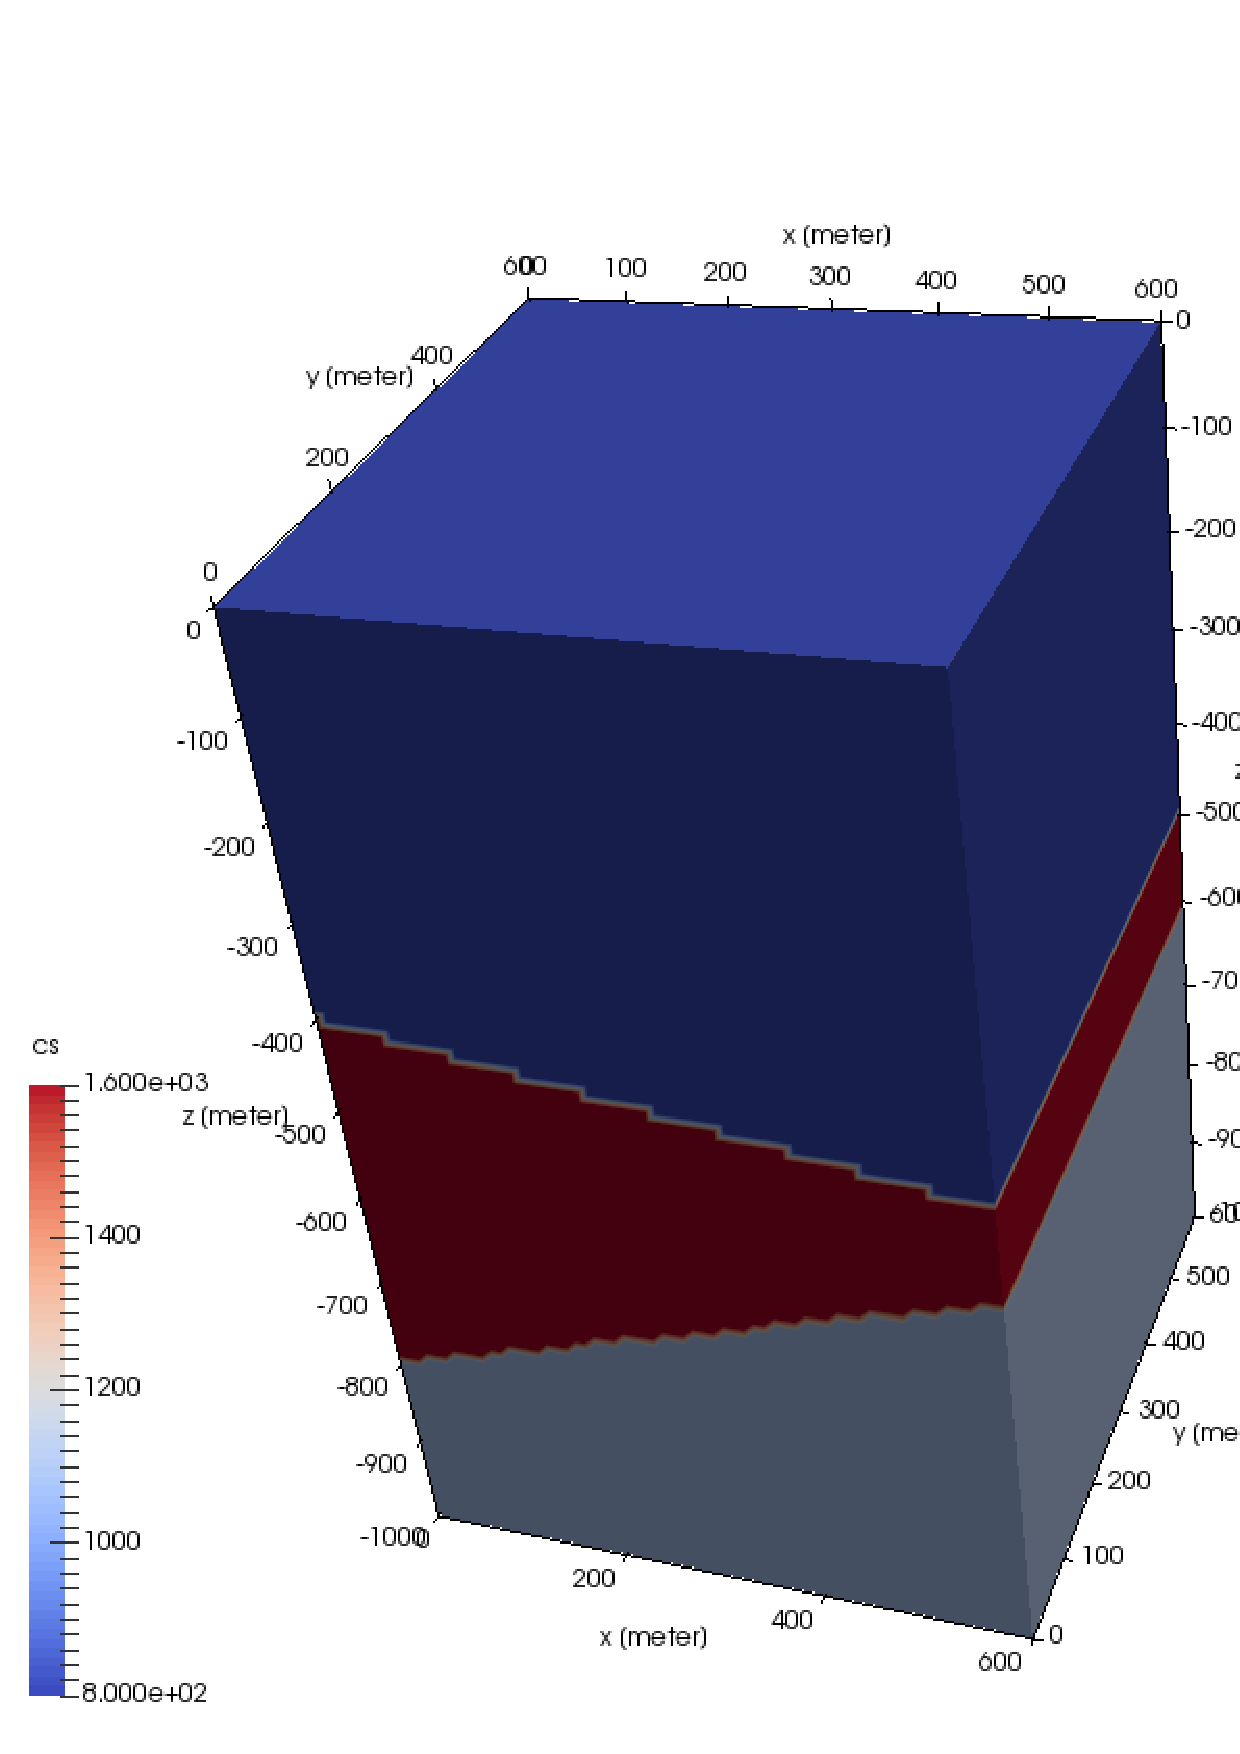
\includegraphics[width=0.49\columnwidth]{wedge3d_cs.png} \hfill
  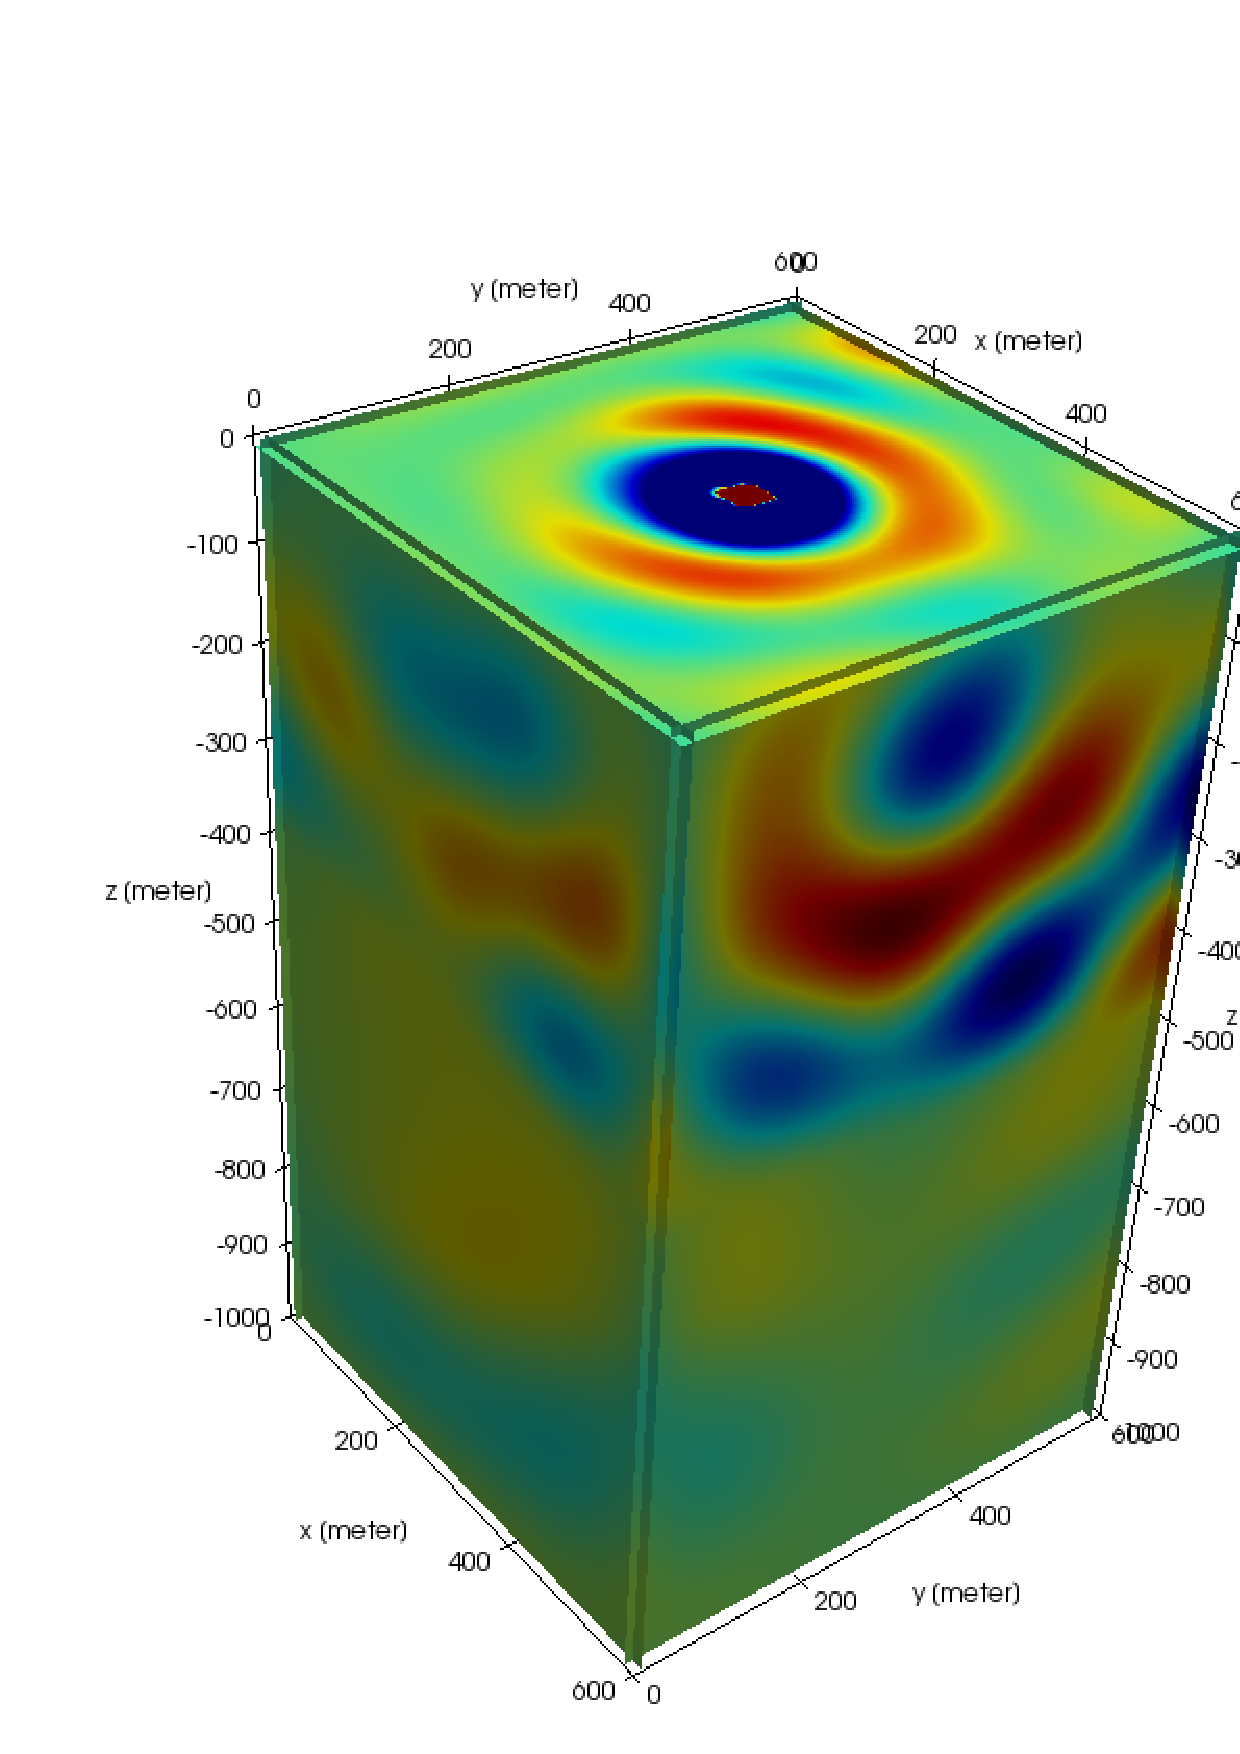
\includegraphics[width=0.49\columnwidth]{wedge3d_f4.png}
  \caption{Left: Parameter configuration of the elastic \texttt{wedge} problem for $d=3$ according to Table \ref{tab_params}. Right: Numerical solution of $\Re(\mathbf{u}_z)$ at $f= 4 Hz$.}\label{fig:3dwegdep1}
\label{fig:wedge3d_par}
\end{figure}

\begin{exper}[A 3D elastic wedge problem] \label{ex:num_3d}
A three-dim- ensional, inhomogeneous elastic wedge problem with physical parameters specified in Table \ref{tab_params} is solved using the SSOR-MSSS preconditioner described in Section \ref{ch_msss3d}.
\end{exper}

Similar to Experiment \ref{exp:freq1}, we consider a constant number of $20$ points per wavelength, and increase the wave frequency from $2$Hz to $4$Hz while doubling the number of grid points in each spatial direction. In Figure \ref{fig:3dwegdep1_conv} we observe a factor of $\sim 4$ which numerically indicates a complexity of $\mathcal{O}(n^5)$ for 3D problems. Moreover, we note that IDR outperforms BiCGStab in terms of number of iterations. The corresponding CPU times are presented in Table \ref{tab:cputime3d}: From the previous analysis, a factor of $\sim 32$ for the overall CPU times is expected since the number of unknowns in three spatial directions is doubled (linear complexity yields a factor of $8$), and Figure \ref{fig:3dwegdep1_conv} motivates an additional factor of $4$ in iteration numbers. 

 \begin{figure}[t]
 \centering
  \includegraphics[width=0.8\columnwidth]{wedge3d_f2_new3.pdf} \\
  \includegraphics[width=0.8\columnwidth]{wedge3d_f4_new2.pdf}
%   \includegraphics[width=0.8\columnwidth]{fig15/slobes.pdf} \\
%   \includegraphics[width=0.8\columnwidth]{fig15/slobes4.pdf}
  \caption{Convergence history of different Krylov methods preconditioned with the SSOR-MSSS preconditioner \eqref{eq:approx_Schur} for the 3D \texttt{wedge} problem of Figure \ref{fig:wedge3d_par}. We indicate (approximate) slopes based on a linear fit of the convergence curves.}\label{fig:3dwegdep1_conv}
 \end{figure}
 
\begin{table}[ht]
  \caption{Total CPU times in seconds corresponding to the convergence plots in Figure \ref{fig:3dwegdep1_conv}. Note that BiCGStab at \mbox{$f=4$ Hz} is stopped after $1,000$ iterations, cf. Figure \ref{fig:3dwegdep1_conv}.}\label{tab:cputime3d}
 \centering
 \begin{tabular}{|l|ccc|}
  \hline
  frequency & BiCGStab & IDR($4$) & IDR($16$)\\
  \hline
  $f=2$ Hz & \phantom{0}\texttt{144.5} & \phantom{00}\texttt{95.5} & \phantom{00}\texttt{91.3}\\
  $f=4$ Hz & \texttt{4430.7} & \texttt{3536.4} & \texttt{3100.5}\\
  \hline
 \end{tabular}
\end{table}

\section{Conclusions}
We present an efficient \textit{hybrid} method for the numerical solution of the inhomogeneous time-harmonic elastic wave equation. We use an incomplete block-LU factorization based on MSSS matrix computations as a preconditioner for IDR($s$). The presented framework further allows to incorporate multiple wave frequencies and multiple source locations in a matrix equation setting \eqref{eq:mateq_approach2}. The suggested MSSS preconditioner is conceptional different for 2D and 3D problems:
\begin{itemize}
 \item We derive an MSSS permutation matrix \eqref{eq:Psi} that transforms the 2D elastic operator into block tridiagonal level-2 MSSS matrix structure. This allows the application of an approximate Schur factorization \eqref{eq:full_Schur}-\eqref{eqn_schur}. In order to a\-chieve linear computational complexity, the involved SSS operations (level-1) are approximated using model order reduction techniques that limit the off-diagonal rank.
 \item A generalization to 3D problems is not straight-forward because no model order reduction algorithms for level-2 MSSS matrices are currently available \cite{QG15}. We therefore suggest the SSOR splitting \eqref{eq:approx_Schur} where off-diagonal blocks are treated as sparse matrices and diagonal blocks resemble a sequence of 2D problems in level-2 MSSS structure.
\end{itemize}

We present a series of numerical experiments on a 2D elastic \texttt{wedge} problem (Figure \ref{fig:wedge2d}) that prove theoretical concepts. In particular, we have numerically shown that a small off-di\-ag\-o\-nal rank $r^\ast \sim 10$ yields a preconditioner such that IDR($s$) converges within very few iterations (Experiment \ref{exp:off_rank}).

Further numerical experiments for 2D elastic problems are performed on the realistic \marmousi data set. The newly derived matrix equation approach shows computational advantages when multiple right-hand sides (Experiment \ref{multiRHS}) and multiple frequencies (Experiment \ref{multifreq}) are solved simultaneously.

In Corollary \ref{mem_3d}, we prove that the MSSS preconditioner has linear memory requirements for 2D and 3D problems. The overall computational complexity is investigated for the case of a constant number of wavelength, i.e. the number of grid points $n$ in one spatial direction in linearly increased with the wave frequency. Numerical experiments show $\mathcal{O}(n^3)$ complexity for 2D (Experiment \ref{exp:freq1}) and $\mathcal{O}(n^5)$ complexity for 3D (Experiment \ref{ex:num_3d}) problems. The 3D preconditioner solves a sequence of 2D problems and can be parallelized in a straight forward way. 

\section*{Acknowledgments}
We would like to thank Joost van Zwieten, co-developer of the open source project \texttt{nutils}\footnote{\url{http://www.nutils.org/}} for helpful discussions concerning the finite element discretization described in Section \ref{ch:discretization}. Shell Global Solutions International B.V. is gratefully acknowledged for financial support of the first author.

% BibTeX users please use one of
%\bibliographystyle{spbasic}      % basic style, author-year citations
\bibliographystyle{spmpsci}      % mathematics and physical sciences
%\bibliographystyle{spphys}       % APS-like style for physics
\bibliography{ref}
% \newpage
\begin{appendix}
\phantom{\LARGE{Appendix}}
\begin{normalsize}
\noindent\textbf{Appendix} \\
\end{normalsize}

\noindent The appendix serves two purposes: We illustrate two basic SSS matrix operations used at 1D level by means of an example computation. At the same time, we complete Algorithm \ref{LU}. For simplicity, we consider the case $n=4$ in Definition \ref{def_sss},
\begin{equation*}%\label{eqn_sss_example}
        A=\begin{bmatrix}
                      D_1 & U_1V_2^\trp & U_1W_2V_3^\trp & U_1W_2W_3V_4^\trp \\
                      P_2Q_1^\trp & D_2 & U_2V_3^\trp & U_2W_3V_4^\trp  \\
                      P_3R_2Q_1^\trp & P_3Q_2^\trp & D_3 & U_3V_4^\trp  \\
                      P_4R_3R_2Q_1^\trp & P_4R_3Q_2^\trp & P_4Q_3^\trp & D_4
                    \end{bmatrix},
\end{equation*}
and refer to standard literature for the more general case.
\section{Inversion of a lower/upper diagonal SSS matrix}
\label{app_invsss}
A lower diagonal SSS matrix in generator form is given by 
\begin{align}
\label{L_sss}
 L = SSS(P_s, R_s, Q_s, D_s, 0, 0, 0), \quad 1 \leq s \leq n,
\end{align}
and we denote $L^{-1}$ via,
\begin{align*}
 L^{-1} = SSS(\underbar{P}_s, \underbar{R}_s, \underbar{Q}_s, \underbar{D}_s, 0, 0, 0), \quad 1 \leq s \leq n.
\end{align*}
Clearly, for $n=4$, the matrix \eqref{L_sss} yields,
\begin{equation*}%\label{eqn_sss_example}
        L=\begin{bmatrix}
                      D_1 & 0 & 0 & 0 \\
                      P_2Q_1^\trp & D_2 & 0 & 0  \\
                      P_3R_2Q_1^\trp & P_3Q_2^\trp & D_3 & 0  \\
                      P_4R_3R_2Q_1^\trp & P_4R_3Q_2^\trp & P_4Q_3^\trp & D_4
                    \end{bmatrix},
\end{equation*}
and we immediately conclude $\underbar{D}_s = D_s^{-1}, s=1,...,4,$ for all diagonal generators of $L^{-1}$.
In Lemma \ref{lu_sss}, we claim that $L^{-1}$ can be computed without increase of the off-diagonal rank, and we illustrate this fact by computing the generators at entry $(2,1)$:
\begin{align*}
 & P_2 Q_1^\trp \underbar{D}_1 + D_2 \underbar{P}_2 \underbar{Q}_1^\trp = 0 \quad \Leftrightarrow \quad \underbar{P}_2 \underbar{Q}_1^\trp \equiv (-D_2^{-1} P_2) (D_1^{-\trp} Q_1)^\trp.
\end{align*}

The computation of $U^{-1}$ in Algorithm \ref{LU} can be done analogously, and we refer to \cite[Lemma 2]{sss_techrep03} for the complete algorithm and the case $n \neq 4$.
\section{Matrix-matrix multiplication in SSS structure}
\label{app_matmulsss}
% {\color{red}How to perform $A \cdot B$? Note that in Lemma \ref{lu_sss} off-diagonal rank won't grow, but in general mat-mat it does!!}
In the final step of Algorithm \ref{LU} we perform the matrix-matrix multiplication  $A^{-1} = U^{-1} \cdot L^{-1}$ with $U^{-1}$ and $L^{-1}$ given in upper/lower diagonal SSS format, cf. Appendix \ref{app_invsss}. In this Section, we illustrate how to perform the SSS matrix-matrix multiplication $C = A \cdot B$ when $n=4$ and $A$ and $B$ are given as,
\begin{align*}
\begin{bmatrix}
    D_1^A & U_1V_2^\trp & U_1W_2V_3^\trp & U_1W_2W_3V_4^\trp \\
    0 & D_2^A & U_2V_3^\trp & U_2W_3V_4^\trp  \\
    0 & 0 & D_3^A & U_3V_4^\trp  \\
    0 & 0 & 0 & D_4^A
    \end{bmatrix},
\begin{bmatrix}
    D_1^B & 0 & 0 & 0 \\
    P_2Q_1^\trp & D_2^B & 0 & 0  \\
    P_3R_2Q_1^\trp & P_3Q_2^\trp & D_3^B & 0  \\
    P_4R_3R_2Q_1^\trp & P_4R_3Q_2^\trp & P_4Q_3^\trp & D_4^B
    \end{bmatrix}.
\end{align*}
The SSS matrix $C$ can then be computed by appropriate block multiplications of the respective generators. For example, the $(3,2)$ entry of the product yields,
\begin{align*}
C_{32} &= 0 \cdot D_2^B + D_3^A P_3 Q_2^\trp + U_3 V_4^\trp P_4 R_3 Q_2^\trp \\
       &= (D_3^A P_3 + U_3 V_4^\trp P_4 R_3) Q_2^\trp \equiv P_3^C (Q_2^C)^\trp
\end{align*}
% \begin{align*}
% C_{32} &= P_3 R_2 Q_1^\trp U_1 V_2^\trp + P_3 Q_2^\trp D_2^B + D_3^A \cdot 0 \\
%        &= P_3 (R_2 Q_1^\trp U_1 V_2^\trp + Q_2^\trp D_2^B) \equiv P_3^C (Q_2^C)^\trp
% \end{align*}

The above computation illustrates on the one hand that the off-diagonal rank does not increase due to the lower/upper diagonal SSS structure of the matrices $A$ and $B$. On the other hand, we note that in general the off-diagonal rank of $C$ will increase due to the non-vanishing term that contains the full-rank generator $D_2^B$. Matrix-matrix multiplication in SSS form is presented in \cite[Theorem~1]{sss_techrep03}.
\end{appendix}

\end{document}
